%%%%%%%%%%%%%%%%%%%%%%%%%%%%%%%%%%%%%%%%%%%%%%%%%%%%%%%%%%%%%%%%%%%%%%
%%%%%%%%%%%%%%%%%%%%%%%%%%%%%%%%%%%%%%%%%%%%%%%%%%%%%%%%%%%%%%%%%%%%%%
%%%%%%%%%%%%%%%%%%%%%%%%%%%%%%%%%%%%%%%%%%%%%%%%%%%%%%%%%%%%%%%%%%%%%%
%%%%%%%%%%%%%%%%%%%%%%%%%%%%%%%%%%%%%%%%%%%%%%%%%%%%%%%%%%%%%%%%%%%%%%
\chapter{Stabilité des systèmes asservis\label{chap-stab}}
%%%%%%%%%%%%%%%%%%%%%%%%%%%%%%%%%%%%%%%%%%%%%%%%%%%%%%%%%%%%%%%%%%%%%%
%%%%%%%%%%%%%%%%%%%%%%%%%%%%%%%%%%%%%%%%%%%%%%%%%%%%%%%%%%%%%%%%%%%%%%
%%%%%%%%%%%%%%%%%%%%%%%%%%%%%%%%%%%%%%%%%%%%%%%%%%%%%%%%%%%%%%%%%%%%%%
%%%%%%%%%%%%%%%%%%%%%%%%%%%%%%%%%%%%%%%%%%%%%%%%%%%%%%%%%%%%%%%%%%%%%%
\minitoc
\newpage

%%%%%%%%%%%%%%%%%%%%%%%%%%%%%%%%%%%%%%%%%%%%%%%%%%%%%%%%%%%%%%%%%%%%%%
%%%%%%%%%%%%%%%%%%%%%%%%%%%%%%%%%%%%%%%%%%%%%%%%%%%%%%%%%%%%%%%%%%%%%%
%%%%%%%%%%%%%%%%%%%%%%%%%%%%%%%%%%%%%%%%%%%%%%%%%%%%%%%%%%%%%%%%%%%%%%
\section{Définitions de la stabilité}
%%%%%%%%%%%%%%%%%%%%%%%%%%%%%%%%%%%%%%%%%%%%%%%%%%%%%%%%%%%%%%%%%%%%%%
%%%%%%%%%%%%%%%%%%%%%%%%%%%%%%%%%%%%%%%%%%%%%%%%%%%%%%%%%%%%%%%%%%%%%%
%%%%%%%%%%%%%%%%%%%%%%%%%%%%%%%%%%%%%%%%%%%%%%%%%%%%%%%%%%%%%%%%%%%%%%

\textbf{Un système est dit stable si à une entrée bornée le système produit une sortie bornée}\footnote{Chez 
nos amis anglo-saxons, on rencontre le concept de BIBO (\og bounded input bounded output\fg)}

\textbf{Un système est dit stable lorsque écarté de sa position d'équilibre, il tend à y revenir}

Ces deux définitions sont équivalentes dans le cas des \glspl{slci}. 

\begin{figure}[!h]
    \centering
\tikzsetnextfilename{stable_1-chap6_ext}
    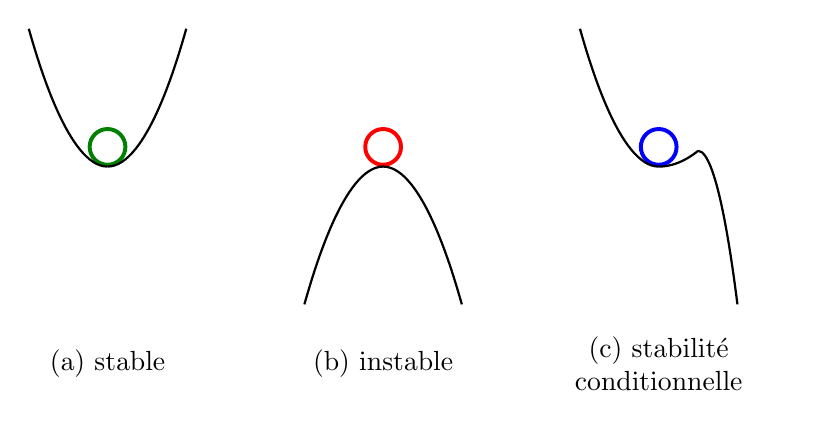
\begin{tikzpicture}
        \draw[green!50!black,line width=0.5mm] (0,0.25) circle (1.5ex);
        \draw[thick] (0,0) parabola (1,1.75) ;
        \draw[thick] (0,0) parabola (-1,1.75) ;
        \node at (0,-2.5) {(a) stable};
        \begin{scope}[xshift=3.5cm]
            \draw[red,line width=0.5mm] (0,0.25) circle (1.5ex);
            \draw[thick] (0,0) parabola (1,-1.75) ;
            \draw[thick] (0,0) parabola (-1,-1.75) ;
            \node at (0,-2.5) {(b) instable};
        \end{scope}
        \begin{scope}[xshift=7cm]
            \draw[blue,line width=0.5mm] (0,0.25) circle (1.5ex);
            \draw[thick] (0,0) parabola (-1,1.75) ;
            \draw[thick] (0,0) parabola (0.5,0.2) ;
            \draw[thick] (0.5,0.2) parabola (1,-1.75) ;
            \node[text width=3cm,align=center] at (0,-2.5) {(c) stabilité\\conditionnelle};
        \end{scope}
    \end{tikzpicture}
\caption{Représentation schématique de la stabilité}
\end{figure}


\begin{center}
\tikzsetnextfilename{stable-chap0_ext}
\begin{tikzpicture}
	\begin{axis}
	[	ticks=none,
        axis line style = thick,
        height=5cm,
        width=5cm,
        axis x line=center,
        axis y line=center,
        xmin=-2,
        xmax=10,
        ymin=-1.5,
        ymax=3.0,
        xlabel={$t$},
        ylabel={$s(t)$},
        xlabel style={below right},
        ylabel style={above left},
	]
	\addplot[signalb,domain=-2:0] {0};
	\addplot[signalb,domain=0:10] {sin(3*deg(x))*exp(-x)+1};
	\draw[dotted,very thick,col1] (axis cs:0,0) -- (axis cs:0,1);
	\end{axis}
\end{tikzpicture}

\end{center}                

\begin{center}
\tikzsetnextfilename{stable2-chap0_ext}
    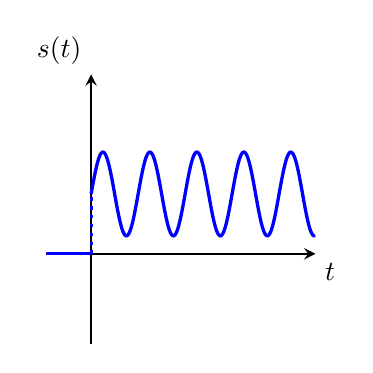
\begin{tikzpicture}
        \begin{axis}[
	ticks=none,
        axis line style = thick,
        height=5cm,
        width=5cm,
        axis x line=center,
        axis y line=center,
        xmin=-2,
        xmax=10,
        ymin=-1.5,
        ymax=3.0,
        xlabel={$t$},
        ylabel={$s(t)$},
        xlabel style={below right},
        ylabel style={above left},
        ]                                                                                                                     
        \addplot [very thick,color=blue,domain=-2:0, samples=101]{0};
	\addplot [very thick,color=blue,domain=0:10, samples=501]{0.7*sin(3*deg(x))+1};
	\draw[dotted,very thick,blue] (axis cs:0,0) -- (axis cs:0,1);
        \end{axis}
    \end{tikzpicture}

\end{center}

\begin{center}
\tikzsetnextfilename{instable-chap0_ext}
    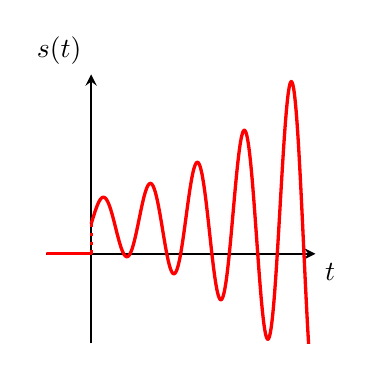
\begin{tikzpicture}
        \begin{axis}[
	ticks=none,
        axis line style = thick,
        height=5cm,
        width=5cm,
        axis x line=center,
        axis y line=center,
        xmin=-2,
        xmax=10,
        ymin=-3,
        ymax=6.0,
        xlabel={$t$},
        ylabel={$s(t)$},
        xlabel style={below right},
        ylabel style={above left},
        ]
        \addplot [very thick,color=red,domain=-2:0, samples=101,unbounded coords=jump]{0};
	\addplot [very thick,color=red,domain=0:10, samples=501,unbounded coords=jump]{0.8*sin(3*deg(x))*exp(0.2*x)+1};
	\draw[dotted,very thick,red] (axis cs:0,0) -- (axis cs:0,1);
        \end{axis}
    \end{tikzpicture}

\end{center}
%%%%%%%%%%%%%%%%%%%%%%%%%%%%%%%%%%%%%%%%%%%%%%%%%%%%%%%%%%%%%%%%%%%%%%
%%%%%%%%%%%%%%%%%%%%%%%%%%%%%%%%%%%%%%%%%%%%%%%%%%%%%%%%%%%%%%%%%%%%%%
%%%%%%%%%%%%%%%%%%%%%%%%%%%%%%%%%%%%%%%%%%%%%%%%%%%%%%%%%%%%%%%%%%%%%%
\section{Critère de stabilité}
%%%%%%%%%%%%%%%%%%%%%%%%%%%%%%%%%%%%%%%%%%%%%%%%%%%%%%%%%%%%%%%%%%%%%%
%%%%%%%%%%%%%%%%%%%%%%%%%%%%%%%%%%%%%%%%%%%%%%%%%%%%%%%%%%%%%%%%%%%%%%
%%%%%%%%%%%%%%%%%%%%%%%%%%%%%%%%%%%%%%%%%%%%%%%%%%%%%%%%%%%%%%%%%%%%%%

\acpl
Réponse temporelle du premier ordre du second ordre ...

\begin{criteria}{Condition fondamentale de stabilité}
    \textbf{Un système est stable si sa fonction de transfert ne possède aucun pôles à partie réelle positive.}
\end{criteria}

\tikzsetnextfilename{stabilite_plan-complexe-chap6_ext}
\clearpage
\thispagestyle{empty}
\begin{landscape}
    \centering
    %\vspace*{\fill}
    \captionsetup{width=1.15\linewidth}
    \begin{figure}[!h]
        \centering
        \begin{tikzpicture}
        \begin{axis}[                                                                                                                     ticks=none,
            width=1.6\textheight,           
            height=\textwidth,    
            axis x line=center,                                                                            
            axis y line=center,
            xmin=-12.5,                                                                                                  
            xmax=12.5,
            ymin=-5,                                                                                                         
            ymax=5,
            xlabel={\LARGE $\Re{(p)}$},
            ylabel={\LARGE $\Im{(p)}$},
            xlabel style={right},
            ylabel style={above},                                                                                       
            ]      
            \draw [white!90!blue,fill=white!95!blue]   (axis cs:-12.5,-5) rectangle (axis cs:0,5);
            \draw [white!90!black,fill=white!90!black] (axis cs:0,-5) rectangle (axis cs:12.5,5);

            \draw [ultra thick,-latex]   (axis cs:-12.5,0) -- (axis cs:12.5,0);
            \draw [ultra thick,-latex]   (axis cs:0,-5) -- (axis cs:0,5);

            \coordinate (pt01) at (axis cs:-6.5,4.5);
            \coordinate (pt02) at (axis cs:6.5,4.5);

            \coordinate (pt1) at (axis cs:-12.5,2.0);
            \addplot[mark=x,black!60!green,ultra thick,only marks,mark size=7pt]  coordinates{ (-11,1.5) (-11,-1.5) } ;      
            \draw[ultra thick,dotted,color=black!60!green] (axis cs:-11,1.5) -- (axis cs:-11,-1.5) ;

            \coordinate (pt2) at (axis cs:-7,1.0);
            \addplot[mark=x,black!10!green,ultra thick,only marks,mark size=7pt]  coordinates{ (-5,0.5) (-5,-0.5) } ;  
            \draw[ultra thick,dotted,color=black!10!green] (axis cs:-5,0.5) -- (axis cs:-5,-0.5) ;

            \coordinate (pt3) at (axis cs:-10.25,-3.0);
            \addplot[mark=x,black!50!red,ultra thick,only marks,mark size=7pt]    coordinates{ (-8,0) } ;             

            \coordinate (pt4) at (axis cs:-4.75,-3.0);
            \addplot[mark=x,red,ultra thick,only marks,mark size=7pt]    coordinates{ (-2,0) } ;                      

            \coordinate (pt5) at  (axis cs:1.25,-5);
            \coordinate (pt52) at (axis cs:1.25,-3);
            \addplot[mark=x,black,ultra thick,only marks,mark size=7pt]  coordinates{ (0,0) } ;                      

            \coordinate (pt6) at (axis cs:1.25,2);
            \coordinate (pt62) at (axis cs:1.25,0);
            \addplot[mark=x,black!50!white,ultra thick,only marks,mark size=7pt]  coordinates{ (0,2) (0,-2) } ;              
            \draw[ultra thick,dotted,color=black!50!white] (axis cs:0,-2) to[bend right] (axis cs:0,2);

            \coordinate (pt7) at (axis cs:8.25,2);
            \addplot[mark=x,blue,ultra thick,only marks,mark size=7pt]   coordinates{ (11,1.5) (11,-1.5) } ;                
            \draw[ultra thick,dotted,color=blue] (axis cs:11,1.5) -- (axis cs:11,-1.5) ;

            \coordinate (pt8) at (axis cs:6.5,-3);
            \addplot[mark=x,orange,ultra thick,only marks,mark size=7pt] coordinates{ (8,0) } ;                  

        \end{axis}


            \node at (pt01) {\textbf{\Large STABLE}};
            \node at (pt02) {\textbf{\Large INSTABLE}};
            % pt1
            \node[anchor=south west] at (pt1) {
                \begin{tikzpicture}
                    \begin{axis}[
                    ticks=none,
                    width=4cm,    
                    height=4cm,    
                    axis x line=center,                                                                            
                    axis y line=center,
                    xmin=-0.5,                                                                                                                    xmax=6.5,
                    ymin=-0.5,                                                                        
                    ymax=2.5,
                    xlabel={$t$},
                    ylabel={$s(t)$},
                    xlabel style={below right},
                    ylabel style={right}
                    ]
                    \addplot [very thick,color=black!60!green,domain=0:10, samples=501,unbounded coords=jump]{1.2*sin(4.5*deg(x))*exp(-0.7*x)};
                    \addplot [thick,dotted,color=black,domain=0:10, samples=501,unbounded coords=jump]{1.2*exp(-0.7*x)+1};
                    \addplot [thick,dotted,color=black,domain=0:10, samples=501,unbounded coords=jump]{-1.2*exp(-0.7*x)+1};
                    \end{axis}
                \end{tikzpicture}
            };

            % pt2
            \node[anchor=south west] at (pt2) {
                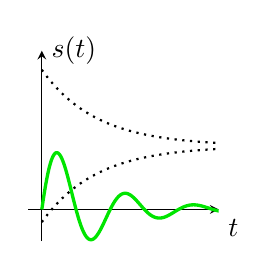
\begin{tikzpicture}
                    \begin{axis}[
                    ticks=none,
                    width=4cm,    
                    height=4cm,    
                    axis x line=center,                                                                            
                    axis y line=center,
                    xmin=-0.5,                                                                                                                    xmax=6.5,
                    ymin=-0.5,                                                                        
                    ymax=2.5,
                    xlabel={$t$},
                    ylabel={$s(t)$},
                    xlabel style={below right},
                    ylabel style={right}
                    ]
                    \addplot [very thick,color=black!10!green,domain=0:10, samples=501,unbounded coords=jump]{1.2*sin(2.5*deg(x))*exp(-0.5*x)};
                    \addplot [thick,dotted,color=black,domain=0:10, samples=501,unbounded coords=jump]{1.2*exp(-0.5*x)+1};
                    \addplot [thick,dotted,color=black,domain=0:10, samples=501,unbounded coords=jump]{-1.2*exp(-0.5*x)+1};
                    \end{axis}
                \end{tikzpicture}
            };
            % pt3
            \node[anchor=south west] at (pt3) {
                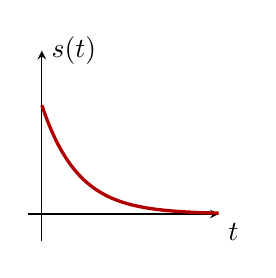
\begin{tikzpicture}
                    \begin{axis}[
                    ticks=none,
                    width=4cm,    
                    height=4cm,    
                    axis x line=center,                                                                            
                    axis y line=center,
                    xmin=-0.5,                                                                                                                    xmax=6.5,
                    ymin=-0.5,                                                                        
                    ymax=3,
                        xlabel={$t$},
                        ylabel={$s(t)$},
                    xlabel style={below right},
                    ylabel style={right}
                    ]
                    \addplot [very thick,color=black!30!red,domain=0:10, samples=501,unbounded coords=jump]{2*exp(-0.75*x)};
                    \end{axis}
                \end{tikzpicture}
            };
            % pt4
            \node[anchor=south west] at (pt4) {
                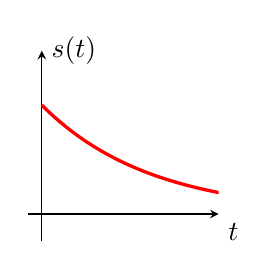
\begin{tikzpicture}
                    \begin{axis}[
                    ticks=none,
                    width=4cm,    
                    height=4cm,    
                    axis x line=center,                                                                            
                    axis y line=center,
                    xmin=-0.5,                                                                                                                    xmax=6.5,
                    ymin=-0.5,                                                                        
                    ymax=3,
                        xlabel={$t$},
                        ylabel={$s(t)$},
                    xlabel style={below right},
                    ylabel style={right}
                    ]
                    \addplot [very thick,color=red,domain=0:10, samples=501,unbounded coords=jump]{2*exp(-0.25*x)};
                    \end{axis}
                \end{tikzpicture}
            };
            % pt5
            \node[anchor=south west] at (pt5) {
                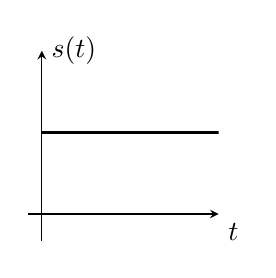
\begin{tikzpicture}
                    \begin{axis}[
                    ticks=none,
                    width=4cm,    
                    height=4cm,    
                    axis x line=center,                                                                            
                    axis y line=center,
                    xmin=-0.5,                                                                                                                    xmax=6.5,
                    ymin=-0.5,                                                                        
                    ymax=3,
                    xlabel={$t$},
                    ylabel={$s(t)$},
                    xlabel style={below right},
                    ylabel style={right}
                    ]
                    \addplot [very thick,color=black,domain=0:10, samples=501,unbounded coords=jump]{1.5};
                    \end{axis}
                \end{tikzpicture}
            };
            % pt52
            \node[anchor=south west] at (pt52) {
                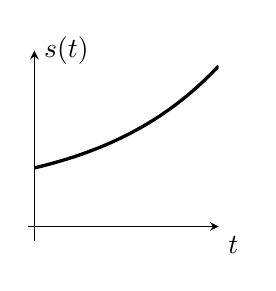
\begin{tikzpicture}
                    \begin{axis}[
                    ticks=none,
                    width=4cm,    
                    height=4cm,    
                    axis x line=center,                                                                            
                    axis y line=center,
                    xmin=-0.5,                                                                                                                    xmax=15,
                    ymin=-0.5,                                                                        
                    ymax=6,
                    xlabel={$t$},
                    ylabel={$s(t)$},
                    xlabel style={below right},
                    ylabel style={right}
                    ]
                    \addplot [very thick,color=black,domain=0:15, samples=501,unbounded coords=jump]{1+exp(0.1*x)};
                    \end{axis}
            \end{tikzpicture}
            };
            % pt6
            \node[anchor=south west] at (pt6) {
                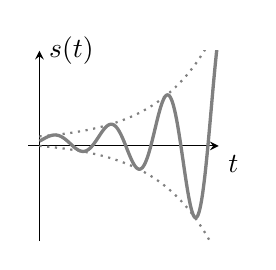
\begin{tikzpicture}
                    \begin{axis}[
                    ticks=none,
                    width=4cm,    
                    height=4cm,    
                    axis x line=center,                                                                            
                    axis y line=center,
                    xmin=-0.5,                                                                                                                    xmax=8,
                    ymin=-20,                                                                        
                    ymax=20,
                    xlabel={$t$},
                    ylabel={$s(t)$},
                    xlabel style={below right},
                    ylabel style={right}
                    ]
              \addplot [very thick,color=black!50!white,domain=0:10, samples=501,unbounded coords=jump]{sin(2.5*deg(x))*exp(0.40*x)+1};
              \addplot [thick,dotted,color=black!50!white,domain=0:10, samples=501,unbounded coords=jump]{ exp(0.4*x)+1};
              \addplot [thick,dotted,color=black!50!white,domain=0:10, samples=501,unbounded coords=jump]{-exp(0.4*x)+1};
                    \end{axis}
                \end{tikzpicture}
            };
            % pt62
            \node[anchor=south west] at (pt62) {
                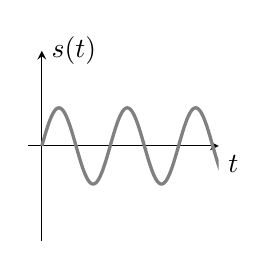
\begin{tikzpicture}
                    \begin{axis}[
                    ticks=none,
                    width=4cm,    
                    height=4cm,    
                    axis x line=center,                                                                            
                    axis y line=center,
                    xmin=-0.5,                                                                                                                    xmax=6.5,
                    ymin=-2.5,                                                                        
                    ymax=2.5,
                    xlabel={$t$},
                    ylabel={$s(t)$},
                    xlabel style={below right},
                    ylabel style={right}
                    ]
                    \addplot [very thick,color=black!50!white,domain=0:10, samples=501,unbounded coords=jump]{sin(2.5*deg(x))};
                    \end{axis}
                \end{tikzpicture}
            };
            % pt7
            \node[anchor=south west] at (pt7) {
                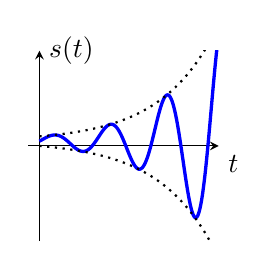
\begin{tikzpicture}
                    \begin{axis}[
                    ticks=none,
                    width=4cm,    
                    height=4cm,    
                    axis x line=center,                                                                            
                    axis y line=center,
                    xmin=-0.5,                                                                                                                    xmax=8.0,
                    ymin=-20,                                                                        
                    ymax=20,
                    xlabel={$t$},
                    ylabel={$s(t)$},
                    xlabel style={below right},
                    ylabel style={right}
                    ]
              \addplot [very thick,color=blue,domain=0:10, samples=501,unbounded coords=jump]{sin(2.5*deg(x))*exp(0.40*x)+1};
              \addplot [thick,dotted,color=black,domain=0:10, samples=501,unbounded coords=jump]{ exp(0.4*x)+1};
              \addplot [thick,dotted,color=black,domain=0:10, samples=501,unbounded coords=jump]{-exp(0.4*x)+1};
                    \end{axis}
              \end{tikzpicture}
            };
            % pt8
            \node[anchor=south west] at (pt8) {
                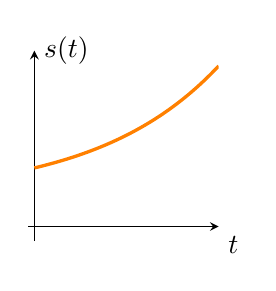
\begin{tikzpicture}
                    \begin{axis}[
                    ticks=none,
                    width=4cm,    
                    height=4cm,    
                    axis x line=center,                                                                            
                    axis y line=center,
                    xmin=-0.5,                                                                                                                    xmax=15,
                    ymin=-0.5,                                                                        
                    ymax=6,
                    xlabel={$t$},
                    ylabel={$s(t)$},
                    xlabel style={below right},
                    ylabel style={right}
                    ]
                    \addplot[very thick,color=orange,domain=0:15,samples=501,unbounded coords=jump]{1+exp(0.1*x)};
                    \end{axis}
                \end{tikzpicture}
            };
        \end{tikzpicture}
    \caption{Stabilité d'un SLCI d'après la carte des pôles de sa fonction de transfert et de leurs
    réponses impulsionnelles.
    (Vert) Deux pôles complexes conjugués. 
    (Rouge) Pôle à partie réel négative. 
    (Gris) Deux pôles complexes conjugués à partie réelle nulle.
    (Noir) Pôle nul.
    (Bleu) Deux pôles complexes conjugués à partie réelle positive.
    (Orange) Pôle à partie réel positive.}
    \end{figure}
%    %\vfill
\end{landscape}

\clearpage
\pagestyle{fancy}
\captionsetup{width=0.8\linewidth}


%%%%%%%%%%%%%%%%%%%%%%%%%%%%%%%%%%%%%%%%%%%%%%%%%%%%%%%%%%%%%%%%%%%%%%
\paragraph{Notion de pôles dominants}
%%%%%%%%%%%%%%%%%%%%%%%%%%%%%%%%%%%%%%%%%%%%%%%%%%%%%%%%%%%%%%%%%%%%%%

%%%%%%%%%%%%%%%%%%%%%%%%%%%%%%%%%%%%%%%%%%%%%%%%%%%%%%%%%%%%%%%%%%%%%%
\paragraph{Système asservi}
%%%%%%%%%%%%%%%%%%%%%%%%%%%%%%%%%%%%%%%%%%%%%%%%%%%%%%%%%%%%%%%%%%%%%%

\begin{center}
\tikzsetnextfilename{asser-chap6_ext}
    \begin{tikzpicture}
        \sbEntree{E}
        \sbComp[5.0]{comp}{E}
        \sbRelier[$E(p)$]{E}{comp}
        \sbBloc[1.5]{B}{$\dfrac{K}{p(p^2+p+3)}$}{comp}
        \sbRelier[$\epsilon$]{comp}{B}
        \sbSortie[5.0]{S}{B}
        \sbRelier[$S(p)$]{B}{S}
    \sbRenvoi{B-S}{comp}{}
\end{tikzpicture}
\end{center}

$$
H_{BF}(p)=\dfrac{N(p)}{D(p)}=\dfrac{a_mp^m+a_{m-1}p^{m-1}+\ldots+a_1p+a_0}{b_np^n+b_{n-1}p^{n-1}+\ldots+b_1p+b_0}
$$

\begin{criteria}{Condition de stabilité d'un système asservi (1)}
    \textbf{Un système asservi est stable si sa fonction de transfert en boucle fermée 
    ne possède aucun pôles à partie réelle positive.}
\end{criteria}


%%%%%%%%%%%%%%%%%%%%%%%%%%%%%%%%%%%%%%%%%%%%%%%%%%%%%%%%%%%%%%%%%%%%%%
\paragraph{Inconvénients de la condition fondamentale}
%%%%%%%%%%%%%%%%%%%%%%%%%%%%%%%%%%%%%%%%%%%%%%%%%%%%%%%%%%%%%%%%%%%%%%

%%%%%%%%%%%%%%%%%%%%%%%%%%%%%%%%%%%%%%%%%%%%%%%%%%%%%%%%%%%%%%%%%%%%%%
%%%%%%%%%%%%%%%%%%%%%%%%%%%%%%%%%%%%%%%%%%%%%%%%%%%%%%%%%%%%%%%%%%%%%%
\subsection{Critère algébrique de Routh}
%%%%%%%%%%%%%%%%%%%%%%%%%%%%%%%%%%%%%%%%%%%%%%%%%%%%%%%%%%%%%%%%%%%%%%
%%%%%%%%%%%%%%%%%%%%%%%%%%%%%%%%%%%%%%%%%%%%%%%%%%%%%%%%%%%%%%%%%%%%%%

Le critère de Routh\footnote{\index{Routh, Edward}Edward John Routh (1831-1907), mathématicien anglais.}
est dit algébrique car il s'établit dirctement sur la fonction de transfert en 
boucle fermée du système asservi. 

Pour appliquer le critère fondamentale de stabilité à cette fonction de transfert,
il nous faut étudier \textbf{le polynôme caractéristique}:
\begin{align}
    D(p)&=0 \nonumber\\
    b_np^n+b_{n-1}p^{n-1}+\ldots+b_1p+b_0 &= 0
\end{align}
pour déterminer si ce polynôme possède des racines toutes à partie réelle 
strictement négative. Les polynômes de ce type sont dits en mathématiques 
de dit de Hurwitz\footnote{\index{Hurwitz, Adolf}Adolf Hurwitz (1859-1919), mathématicien allemand.}\footnote{Un polynôme de 
Hurwitz est un polynôme à coefficients 
réels dont les racines sont toutes à partie réelle strictement négative.}.
C'est pourquoi le critère suivant est également connu sous le nom de \textbf{critère de Routh-Hurwitz}.

Il est possible de conclure sur la nature des racines d'un polynôme 
en étudiant ses coefficients. Le critère de Routh-Hurwitz se base sur cette propriété en 
posant deux conditions pour établir qu'un polynôme est un polynôme de Hurwitz.
Dans le cas de l'application de la stabilité des systèmes linéaires asservis, la première condition s'énonce 
de la façon suivante :
\begin{criteria}{Condition nécessaire de Routh-Hurwitz }
    \textbf{Un système asservi d'ordre $n$ est stable en boucle fermée 
    si tous les coefficients ($b_i\forall i\neq n$) de son équation caractéristique 
    sont de même signe que $b_n$.}
\end{criteria}

Cette condition nécessaire s'avère suffisante si le système est du premier ou du second ordre.
Pour un ordre supérieur il faut construire le tableau de Routh à partir des coefficients de $D(p)$,
pour appliquer une condition supplémentaire. 

%%%%%%%%%%%%%%%%%%%%%%%%%%%%%%%%%%%%%%%%%%%%%%%%%%%%%%%%%%%%%%%%%%%%%%
\subsubsection{Tableau de Routh}
%%%%%%%%%%%%%%%%%%%%%%%%%%%%%%%%%%%%%%%%%%%%%%%%%%%%%%%%%%%%%%%%%%%%%%
Dans le cas où la condition nécessaire est respectée et $n>2$, il faut constuire le \textbf{tableau de Routh}
à partir des coefficients de l'équation caractéristique de la fonction de transfert en boucle fermée.

Le tableau de Routh est constitué de $n$ lignes et de $k$ colonnes 
où $k=n/2+1$\footnote{On réalise ici une division entière. Par exemple 
si $n=5$, $k=2+1=3$ et si $n=6$, $k=3+1=4$}. L'élément $A_{ij}$ correspond 
à l'élément de la $i$-ème ligne et $j$-ème colonne.
\[
\begin{matrix}
    p^n    \\
    p^{n-1}\\
    p^{n-2}\\
    p^{n-3}\\
    \vdots \\
    p^1    \\
    p^0    \\
\end{matrix}
\begin{vmatrix}
    A_{11}     & A_{12}     & A_{13}     & \cdots & A_{1(k-1)}     & A_{1k}      \\
    A_{21}     & A_{22}     & A_{23}     & \cdots & A_{2(k-1)}     & A_{2k}      \\
    A_{31}     & A_{32}     & A_{33}     & \cdots & A_{3(k-1)}     & A_{3k}      \\
    A_{41}     & A_{42}     & A_{43}     & \cdots & A_{4(k-1)}     & A_{4k}      \\
    \vdots     & \vdots     & \vdots     & A_{ij} & \vdots         & \vdots      \\
    A_{(n-1)1} & A_{(n-1)2} & A_{(n-1)3} & \cdots & A_{(n-1)(k-1)} & A_{(n-1)k}  \\
    A_{n1}     & A_{n2}     & A_{n3}     & \cdots & A_{n(k-1)}     & A_{nk}
\end{vmatrix}
\]

Les deux premières lignes du tableau sont directement construites à partir des coefficients de $D(p)$.
\[
    \textbf{paire}\qquad\quad
\begin{matrix}
    p^n    \\
    p^{n-1}\\
    \hline
    \vdots \\
\end{matrix}
\begin{vmatrix}
    b_n       & b_{n-2}    & b_{n-4}    & \cdots & b_2            & b_0         \\
    b_{n-1}   & b_{n-3}    & b_{n-5}    & \cdots & b_1            & 0           \\
    \hline
    \vdots    & \vdots     & \vdots     & \vdots & \vdots         & \vdots      \\
    \end{vmatrix}
\]
si $n$ est impaire la dernière colonne de la seconde ligne est non-nulle:
\[
    \textbf{impaire}\qquad
\begin{matrix}
    p^n    \\
    p^{n-1}\\
    \hline
    \vdots \\
\end{matrix}
\begin{vmatrix}
    b_n       & b_{n-2}    & b_{n-4}    & \cdots & b_3            & b_1         \\
    b_{n-1}   & b_{n-3}    & b_{n-5}    & \cdots & b_2            & b_0         \\
    \hline
    \vdots    & \vdots     & \vdots     & \vdots & \vdots         & \vdots      \\
    \end{vmatrix}
\]

Les éléments de la troisième ligne sont construits à partir du 
déterminant\footnote{Le déterminant d'une matrice 2$\times$2 est tel que 
$\begin{vmatrix} a & b \\ c & d \end{vmatrix}=ad-bc$} des élements des deux premières lignes.
\[
\begin{matrix}
    p^n    \\
    p^{n-1}\\
    \hline
    p^{n-2}\\
    \vdots \\
\end{matrix}
\begin{vmatrix}
    \textcolor{red}{b_n}       & \textcolor{red}{b_{n-2}}    & b_{n-4}    & \cdots & b_3            & b_1         \\
    \textcolor{red}{b_{n-1}}   & \textcolor{red}{b_{n-3}}    & b_{n-5}    & \cdots & b_2            & b_0         \\
    \hline
    %\hmm{A_{31}}{red}   & A_{32}     & A_{33}     & \cdots & \cdots         & \cdots      \\
    A_{31}  & A_{32}     & A_{33}     & \cdots & \cdots         & \cdots      \\
    \vdots    & \vdots     & \vdots     & \vdots & \vdots         & \vdots      \\
\end{vmatrix}
\Rightarrow
A_{31}=-\dfrac{1}{b_{n-1}}\begin{vmatrix} b_{n}  & b_{n-2} \\ b_{n-1} & b_{n-3}\end{vmatrix}
\]

\[
\begin{matrix}
    p^n    \\
    p^{n-1}\\
    \hline
    p^{n-2}\\
    \vdots \\
\end{matrix}
\begin{vmatrix}
    \textcolor{blue}{b_n}       & b_{n-2}    & \textcolor{blue}{b_{n-4}}    & \cdots & b_3            & b_1         \\
    \textcolor{blue}{b_{n-1}}   & b_{n-3}    & \textcolor{blue}{b_{n-5}}    & \cdots & b_2            & b_0         \\
    \hline
    %A_{31}    & \hmm{A_{32}}{blue}     & A_{33}     & \cdots & \cdots         & \cdots      \\
    A_{31}    & A_{32}     & A_{33}     & \cdots & \cdots         & \cdots      \\
    \vdots    & \vdots     & \vdots     & \vdots & \vdots         & \vdots      \\
\end{vmatrix}
\Rightarrow
A_{32}=-\dfrac{1}{b_{n-1}}\begin{vmatrix} b_{n}  & b_{n-4} \\ b_{n-1} & b_{n-5}\end{vmatrix}
\]

On construit de la même manière la quatrième ligne :
\[
\begin{matrix}
    p^n    \\
    p^{n-1}\\
    \hline
    p^{n-2}\\
    p^{n-3}\\
    \vdots \\
\end{matrix}
\begin{vmatrix}
    b_n       & b_{n-2}    & b_{n-4}    & \cdots & b_3            & b_1         \\
     \textcolor{red}{b_{n-1}}   &  \textcolor{red}{b_{n-3}}    & b_{n-5}    & \cdots & b_2            & b_0         \\
    \hline
     \textcolor{red}{A_{31}}     &  \textcolor{red}{A_{32}}    & A_{33}    & \cdots & \cdots         & \cdots      \\
    %\hmm{A_{41}}{red}      & A_{42}     & A_{43}    & \cdots & \cdots         & \cdots      \\
    A_{41}      & A_{42}     & A_{43}    & \cdots & \cdots         & \cdots      \\
    \vdots    & \vdots     & \vdots     & \vdots & \vdots         & \vdots      \\
    \end{vmatrix}
\Rightarrow
A_{41}=-\dfrac{1}{A_{31}}\begin{vmatrix} A_{21} & A_{22} \\ A_{31} & A_{22} \end{vmatrix}
\]

\[
\begin{matrix}
    p^n    \\
    p^{n-1}\\
    \hline
    p^{n-2}\\
    p^{n-3}\\
    \vdots \\
\end{matrix}
\begin{vmatrix}
    b_n       & b_{n-2}    & b_{n-4}    & \cdots & b_3            & b_1         \\
     \textcolor{blue}{b_{n-1}}   &  b_{n-3}    & \textcolor{blue}{b_{n-5}}    & \cdots & b_2            & b_0         \\
    \hline
     \textcolor{blue}{A_{31}}     &  A_{32}    & \textcolor{blue}{A_{33}}    & \cdots & \cdots         & \cdots      \\
    %A_{41}      & \hmm{A_{42}}{blue}     & A_{43}    & \cdots & \cdots         & \cdots      \\
    A_{41}      & A_{42}     & A_{43}    & \cdots & \cdots         & \cdots      \\
    \vdots    & \vdots     & \vdots     & \vdots & \vdots         & \vdots      \\
    \end{vmatrix}
\Rightarrow
A_{42}=-\dfrac{1}{A_{31}}\begin{vmatrix} A_{21} & A_{23} \\ A_{31} & A_{33} \end{vmatrix}
\]

Et ainsi de suite jusque la dernière ligne du tableau. 

La formule générale pour obtenir l'élément $A_{ij}$ est alors :

\begin{bequation}[ams align]
A_{ij}=-\dfrac{1}{A_{(i-1)1}}\begin{vmatrix} A_{(i-2)1} & A_{(i-2)(j+1)} \\ A_{(i-1)1} & A_{(i-1)(j+1)} \end{vmatrix}
\end{bequation}

\newcommand*{\DoTikzmarkU}[1]{%
\tikzset{external/export next=false}
    \tikz[remember picture] \coordinate[shift={(-1ex,1.75ex)}](#1);%
}
\newcommand*{\DoTikzmarkD}[1]{%
\tikzset{external/export next=false}
    \tikz[remember picture] \coordinate[shift={(-1ex,-0ex)}](#1);%
}

\renewcommand*{\colrow}[3][]{%
\tikzset{external/export next=false}
  \tikz[overlay,remember picture, line width=40pt]
    \draw[shorten >=-1.25em, shorten <=-.5em, #1] (#2.north)--(#3.north);
}                                                                                                                             
Le critère s'applique sur la première colonne ainsi construit dite \textbf{colonne des pivots} du tableau de Routh. 
\[
\begin{matrix}
    p^n    \\
    p^{n-1}\\
    p^{n-2}\\
    p^{n-3}\\
    \vdots \\
    p^1    \\
    p^0    \\
\end{matrix}
\begin{vmatrix}
    b_n\DoTikzmarkU{n1}  & b_{n-2}    & b_{n-4}    & \cdots & b_2        & b_0         \\
    b_{n-1}                 & b_{n-3}    & b_{n-5}    & \cdots & b_1        & 0           \\
    A_{31}                  & A_{32}     & A_{33}     & \cdots & A_{3(k-1)} & 0           \\
    A_{41}                  & A_{42}     & A_{43}     & \cdots & 0          & 0           \\
    \vdots                  & \vdots     & \vdots     & \vdots & \vdots     & 0           \\
    A_{(n-1)1}              & A_{(n-1)2} & 0          & \cdots & 0          & 0           \\
    b_0\DoTikzmarkD{n2}  & 0          & 0          & \cdots & 0          & 0
\end{vmatrix}
\]
\colrow[green,opacity=.2]{n1}{n2}

\begin{criteria}{Critère de Routh-Hurtwitz}
    \textbf{Un système asservi est stable en boucle fermée
            si tous les termes de la colonne des pivots 
            du tableau de Routh du polynôme caractéristique 
            de la fonction de transfert en boucle fermée sont de même signes.}
\end{criteria}

%%%%%%%%%%%%%%%%%%%%%%%%%%%%%%%%%%%%%%%%%%%%%%%%%%%%%%%%%%%%%%%%%%%%%%
\paragraph{Remarques:}
%%%%%%%%%%%%%%%%%%%%%%%%%%%%%%%%%%%%%%%%%%%%%%%%%%%%%%%%%%%%%%%%%%%%%%
Le nombre de changement de signe, nous donne le nombre de pôles à partie réelle positives (instables)
de la fonction de transfert en boucle fermée.


\paragraph{Propriétés du tableau de Routh}

Nous énonçons ici quelques propriétés du tableau de Routh 
pour faciliter ou permettre l'application du critère dans 
des cas particuliers~\cite{Ostertag}. 

\begin{itemize}
    \item Pour simplifier les calculs, il est possible de factorisée par un entier une ligne du tableau.
    \item Dans le cas où le tableau présente un zéro dans la première 
          colonne, il est possible de remplacer par une variable $\epsilon$, et de prendre la limite
          lorsque $\epsilon\rightarrow 0^+$ ou $\epsilon\rightarrow 0^-$ selon le signe de la colonne des pivots
          qui respecterait le critère.
    \item Une ligne de zéros pour les coefficients de l'avant-dernière ligne du tableau de
    Routh indique que le polynôme du dénominateur de la fonction de transfert 
        possède une paire de pôles, qui sont racines de l'équation auxiliaire :
    $$
    Ap^2+B=0
    $$
    où $A$ et $B$ sont les coefficients de la ligne précédente du tableau. On peut alors 
    continuer le tableau en remplaçant la
    ligne de coefficients nuls par les coefficients de la dérivée de l'équation auxiliaire.
    
    Une ligne de zéro implique la présence d'une paire de racines imaginaires pures
    donnant lieu à une forme sinuso\"idale dans la réponse transitoire.
    Le système diverge en oscillant s'il y a au moins une racine à partie réelle positive,
    ou il converge vers des oscillations entretenues si les autres racines ont toutes une partie réelle négative.

\end{itemize}

%%%%%%%%%%%%%%%%%%%%%%%%%%%%%%%%%%%%%%%%%%%%%%%%%%%%%%%%%%%%%%%%%%%%%%
\subsubsection{Exemple d'application du critère de Routh-Hurwitz}
%%%%%%%%%%%%%%%%%%%%%%%%%%%%%%%%%%%%%%%%%%%%%%%%%%%%%%%%%%%%%%%%%%%%%%

La particularité du critère de Routh-Hurwitz est de permettre d'étudier les conditions
de stabilité d'un système en fonction des paramètres de la fonction de 
transfert en boucle ouverte.

Dans l'exemple ci-dessous, nous allons considérer un système asservi caractérisé 
par fonction de transfert en boucle ouverte défini par un gain $K$
dont l'on souhaite déterminer la valeur pour assurer la stabilité du système en boucle fermée.

Soit un système asservi défini par le schéma-bloc suivant :
\begin{center}
\tikzsetnextfilename{routh_exemple-chap6_ext}
    \begin{tikzpicture}
        \sbEntree{E}
        \sbComp[5.0]{comp}{E}
        \sbRelier[$E(p)$]{E}{comp}
        \sbBloc[1.5]{B}{$\dfrac{K}{p(p^2+p+3)}$}{comp}
        \sbRelier[$\epsilon$]{comp}{B}
        \sbSortie[5.0]{S}{B}
        \sbRelier[$S(p)$]{B}{S}
    \sbRenvoi{B-S}{comp}{}
\end{tikzpicture}
\end{center}

La fonction de transfert en boucle fermée $H_{BF}(p)$ s'écrit :
$$
H_{BF}(p)=\dfrac{H_{BO}(p)}{1+H_{BO}(p)}=\dfrac{K}{p^3+p^2+3p+K}.
$$

L'équation caractéristique $D(p)$ de $H_{BF}$ est donc 
$$
D(p)=p^3+p^2+3p+K,
$$
Nous constatons que le système est d'ordre 3 de coefficients :
\begin{align*}
    b_3&=1\\
    b_2&=1\\
    b_1&=3\\
    b_0&=K
\end{align*}
Le critère nécessaire de Routh est donc respecté pour $K>0$. L'équation caractéristique 
étant d'ordre 3, il nous faut construire le tableau de Routh, afin de vérifier le critère supplémentaire :

\[
\begin{matrix}
    p^3 \\
    p^2 \\
    \hline
    p^1 \\
    p^0 \\
\end{matrix}
\begin{vmatrix}
     1      & 3  \\
     1      & K  \\
    \hline
    A_{31}  & 0  \\
    A_{41}  & 0    
    \end{vmatrix}
\]

$$
A_{31}=-\begin{vmatrix}1 & 3 \\ 1 & K\end{vmatrix}=3-K
$$

$$
A_{41}=-\dfrac{1}{A_{31}}\begin{vmatrix} 1 & K \\ A_{31} & 0 \end{vmatrix}=K
$$
\renewcommand*{\DoTikzmarkU}[1]{%
\tikzset{external/export next=false}
    \tikz[remember picture] \coordinate[shift={(-0.6ex,1.75ex)}](#1);%
}
\renewcommand*{\DoTikzmarkD}[1]{% 
\tikzset{external/export next=false}
    \tikz[remember picture] \coordinate[shift={(-0.6ex,-6ex)}](#1);%
}
\renewcommand*{\colrow}[3][]{%
\tikzset{external/export next=false}
  \tikz[overlay,remember picture, line width=30pt]
  \draw[shorten >=-.5em, shorten <=-.5em, #1] (#2.north)--(#3.north);
}
\[
\begin{matrix}
    p^3 \\
    p^2 \\
   % \hline
    p^1 \\
    p^0 \\
\end{matrix}
\begin{vmatrix}
    1\DoTikzmarkU{n3}   & 3  \\
    1\DoTikzmarkD{n4}     & K  \\
   % \hline
    3-K                      & 0  \\
    K                        & 0    
    \end{vmatrix}
\]
\colrow[green,opacity=.2]{n3}{n4}

La colonne des pivots sont tous de même signe si $3-K>0$ et $K>0$ (déjà établie par la condition nécessaire de Routh).
La condition sur $K$ pour que le système soit stable en boucle fermée est donc :
\[
0<K<3
\]

%%%%%%%%%%%%%%%%%%%%%%%%%%%%%%%%%%%%%%%%%%%%%%%%%%%%%%%%%%%%%%%%%%%%%%
%%%%%%%%%%%%%%%%%%%%%%%%%%%%%%%%%%%%%%%%%%%%%%%%%%%%%%%%%%%%%%%%%%%%%%
\subsection{Critère graphique du revers}
%%%%%%%%%%%%%%%%%%%%%%%%%%%%%%%%%%%%%%%%%%%%%%%%%%%%%%%%%%%%%%%%%%%%%%
%%%%%%%%%%%%%%%%%%%%%%%%%%%%%%%%%%%%%%%%%%%%%%%%%%%%%%%%%%%%%%%%%%%%%%

Routh s'applique sur la fonction de transfert en boucle fermée. 
Les critères graphiques que nous allons maintenant établir 
permettent d'étudier la stabilité du système en boucle fermée en considérant le système en boucle ouverte.

Pour celà considèrons la boucle de contre réaction unitaire 
pour l'asservissement d'un système de fonction de transfert $H(p)$, telle que : 
\begin{center}
\tikzsetnextfilename{sb_revers-chap6_ext}
    \begin{tikzpicture}
    \sbEntree{E}
    \sbComp[5.0]{comp}{E}
        \sbRelier[$E(p)$]{E}{comp}
        \sbBloc[1.5]{B}{$H(p)$}{comp}
        \sbRelier[$\epsilon$]{comp}{B}
        \sbSortie[5.0]{S}{B}
        \sbRelier[$S(p)$]{B}{S}
    \sbRenvoi{B-S}{comp}{}
\end{tikzpicture}
\end{center}

la fonction de transfert en boucle ouverte $H_{BO}(p)$ est simplement donné par $H(p)$, et comme nous l'avons 
déjà rencontré à plusieurs occasions, la fonction de transfert en boucle fermée $H_{BF}(p)$ est égale à 
$$
H_{BF}(p)=\dfrac{N(p)}{D(p)}=\dfrac{H_{BO}(p)}{1+H_{BO}(p)},
$$
\'Etudier les pôles de l'équation caractéristique $D(p)=0$ est équivalent à étudier l'équation $1+H_{BO}(p)=0$, ou encore
$$
D(p)=0\Leftrightarrow1+H_{BO}(p)=0\Leftrightarrow H_{BO}(p)=-1
$$
Il est alors possible d'étudier la fonction de transfert en boucle ouverte par rapport au \textbf{point critique}\index{Point critique}
du plan complexe $(-1,0)$ de $H_{BO}(p)$.
Remarquons que les zéros de $1+H_{BO}(p)$ sont les pôles de la fonction de transfert en boucle fermée $H_{BF}(p)$ et
que les pôles de $1+H_{BO}(p)$ co\"incident avec les pôles de $H_{BO}(p)$.
Il est donc possible de réinterpréter la condition stabilité d'un système asservi :

\begin{criteria}{Condition de stabilité d'un système asservi (2)}
    \textbf{Un système asservi est stable en boucle fermée si sa fonction de transfert 
    en boucle ouverte ne possède aucun \emph{zéros} à partie réelle positive.}
\end{criteria}

Nous allons établir un critère que nous pourrons appliquer sur la réponse harmonique et 
ses différentes représentations graphiques.

Supposons le système asservi précédent décrit 
par la fonction de transfert en boucle ouverte $H_{BO}(p)$. Par définition cette fonction 
de transfert est le rapport de la sortie $S(p)$ sur l'écart $\epsilon(p)$ que l'on souhaite minimiser.

$$
S(p)=H_{BO}(p)\epsilon(p)
$$

Considérons une entrée $e(t)$ sinuso\"idale de la forme :
$$
e(t)=E_0\sin{\omega t}
$$
au premier instant, on a alors 
$$
\epsilon(t)=E_0\sin{\omega t}
$$
en régime permanent la sortie est alors de la forme (c.f~\cref{chap-anafreq}) :
$$
s(t)=E_0|H_{BO}(\jw)|\sin{(\omega t+\phi)}
$$

l'écart $\epsilon(t)=e(t)-s(t)$ est maximum pour une sortie en opposition de phase.
Il existe donc une pulsation $\omega_p$ pour laquelle:
\begin{align*}
    \phi=\arg{H_{BO}(j\omega_p)}=-\pi\\
    |H_{BO}(j\omega_p)|=K    
\end{align*}

Pour cette pulsation et ce déphasage: 
$$
S(p)=-K\epsilon(p)
$$
on a alors :
$$
H_{BO}(p)=-K
$$

L'écart dans le domaine de Laplace devient:
\begin{align*}
    \epsilon(p)&=E(p)-S(p)\\
    \epsilon(p)&=E(p)+K\epsilon(p)
\end{align*}

Remplaçons à nouveau $\epsilon(p)$ par sa définition (pour simuler une deuxième boucle) : 
\begin{align*}
    \epsilon(p)&=E(p)+K(E(p)-S(p))=E(p)(1+K)+K^2\epsilon(p)
\end{align*}
et ainsi de suite :
\begin{align*}
    \epsilon(p)&=E(p)(1+K)+K^2\left(E(p)-S(p)\right)=E(p)(1+K+K^2)+K^3\epsilon(p)\\
\end{align*}
on obtient après $n$ substitutions :
$$
\epsilon(p)=E(p)\sum_{i=0}^{n}K^i+K^n\epsilon(p)
$$
La somme diverge si $K\leq1$ et converge si $K<1$. Autrement dit le système est stable 
en boucle fermée pour $|H_{BO}(\jw)|<1$.

Nous pouvons donc énoncer le critère de stabilité dit du revers :

\begin{criteria}{Critère de stabilité du revers}
    \textbf{Un système est stable en boucle fermée si lorque le déphasage en boucle 
    ouverte est de -180\degree~le module $|H_{BO}(\jw)|$ est strictement inférieur à 1.}
    Pour $\omega_p$ telle que $\phi=\arg{\left(H_{BO}(j\omega_p)\right)}=-\pi$ stable 
    si  $|H_{BO}(j\omega_p)|<1$ ou $20\log{|H_{BO}(j\omega_p)|}<0$ 
\end{criteria}

Dans le plan complexe, un  déphasage de -180\degree~et un module de 1 
correspond au point critique de coordonnées $(1,0)$.

Nous allons maintenant voir comment appliquer ce critère aux différentes représentations graphiques
de la réponse harmonique.

\newpage
%%%%%%%%%%%%%%%%%%%%%%%%%%%%%%%%%%%%%%%%%%%%%%%%%%%%%%%%%%%%%%%%%%%%%%
\subsubsection{Critère du revers dans le plan de Nyquist}
%%%%%%%%%%%%%%%%%%%%%%%%%%%%%%%%%%%%%%%%%%%%%%%%%%%%%%%%%%%%%%%%%%%%%%

Pour énoncer le critère du revers dans le plan de Nyquist. Il nous faut tracer
le lieu de Nyquist de la fonction de transfert en boucle ouverte et observer comment il 
se comporte par rapport au point critique de coordonnées (-1,0) dans le plan complexe de $H_{BO}(\jw)$.
La~\cref{fig-nyquist_revers} présente les lieux de Nyquist de trois systèmes: stable, instable et critique.
Observons que dans le cas stable, le lieu de déphasage $\phi=-\pi$ (c.a.d lorsque le lieu coupe l'axe des réels négatifs), 
le module ou le gain naturel $G(\omega)$ (ou encore la distance à l'origine) est inférieur à 1. 
Dans le cas instable ce gain est supérieur à 1. Nous appelerons critique le système dont le lieu de Nyquist passe par le
point critique de oordonnées (-1,0).

\begin{figure}[!h]
\begin{center}
\tikzsetnextfilename{critere_revers_nyquist-chap6_ext}
\begin{tikzpicture}
\begin{axis}
    [
    height=9cm,
    width=8cm,
    axis lines = center,
    ticks=none,
    axis line style = thick,
    enlargelimits=false,
    xlabel=$\Re{H_{BO}(\jw)}$,
    ylabel=$\Im{H_{BO}(\jw)}$,
    xlabel style={below right},
    ylabel style={right},
    ymin=-4,
    ymax=2.2,
    xmin=-2.25,
    xmax=0.5,
    clip=false
    ]     
    \addplot [black, mark = *] coordinates {( -1, 0)} {};
    \node [above left,xshift=1ex]  at (axis cs:  -1, 0)   {$(-1,0)$};                
    
    % instable
    \def\xu{-0.2}
    \def\yu{1.75}
    \def\xd{-2.25}
    \def\yd{1.75}
    \def\xt{-2.25}
    \def\yt{-4}
    \addplot [-latex,red,thick,domain=1:0.8,samples=25]
    ({(1-x)*((1-x)*(x*\xu)+x*((1-x)*\xu+x*\xd))+x*((1-x)*((1-x)*\xu+x*\xd)+x*((1-x)*\xd+x*\xt))},
    {(1-x)*((1-x)*(x*\yu)+x*((1-x)*\yu+x*\yd))+x*((1-x)*((1-x)*\yu+x*\yd)+x*((1-x)*\yd+x*\yt))});
    \addplot [-latex,red,thick,domain=0.81:0.5,samples=25]
    ({(1-x)*((1-x)*(x*\xu)+x*((1-x)*\xu+x*\xd))+x*((1-x)*((1-x)*\xu+x*\xd)+x*((1-x)*\xd+x*\xt))},
    {(1-x)*((1-x)*(x*\yu)+x*((1-x)*\yu+x*\yd))+x*((1-x)*((1-x)*\yu+x*\yd)+x*((1-x)*\yd+x*\yt))});
    \addplot [-latex,red,thick,domain=0.51:0.3,samples=25]
    ({(1-x)*((1-x)*(x*\xu)+x*((1-x)*\xu+x*\xd))+x*((1-x)*((1-x)*\xu+x*\xd)+x*((1-x)*\xd+x*\xt))},
    {(1-x)*((1-x)*(x*\yu)+x*((1-x)*\yu+x*\yd))+x*((1-x)*((1-x)*\yu+x*\yd)+x*((1-x)*\yd+x*\yt))});
    \addplot [red,thick,domain=0.31:0,samples=25]
    ({(1-x)*((1-x)*(x*\xu)+x*((1-x)*\xu+x*\xd))+x*((1-x)*((1-x)*\xu+x*\xd)+x*((1-x)*\xd+x*\xt))},
    {(1-x)*((1-x)*(x*\yu)+x*((1-x)*\yu+x*\yd))+x*((1-x)*((1-x)*\yu+x*\yd)+x*((1-x)*\yd+x*\yt))});

    \node [red,left]  at (axis cs:  -2.3, -3.5)   {\textbf{instable}};                
    \addplot [red, mark = *]  coordinates   {(-1.7,0)} {};
    \draw[dblarw={red}{2pt}{2pt}] (0,1.9) -- node[midway,above]  {$G(\omega)>1$} (-1.7,1.9) ;
    \draw[red,dashed] (-1.7,1.9)--(-1.7,0);

    % critique 
    \def\xu{-0.5}
    \def\yu{0.8}
    \def\xd{-1.506}
    \def\yd{0.8}
    \def\xt{-1.495}
    \def\yt{-4}
    \addplot [-latex,blue,thick,domain=1:0.8,samples=50]
    ({(1-x)*((1-x)*(x*\xu)+x*((1-x)*\xu+x*\xd))+x*((1-x)*((1-x)*\xu+x*\xd)+x*((1-x)*\xd+x*\xt))},
    {(1-x)*((1-x)*(x*\yu)+x*((1-x)*\yu+x*\yd))+x*((1-x)*((1-x)*\yu+x*\yd)+x*((1-x)*\yd+x*\yt))});
    \addplot [-latex,blue,thick,domain=0.81:0.3,samples=25]
    ({(1-x)*((1-x)*(x*\xu)+x*((1-x)*\xu+x*\xd))+x*((1-x)*((1-x)*\xu+x*\xd)+x*((1-x)*\xd+x*\xt))},
    {(1-x)*((1-x)*(x*\yu)+x*((1-x)*\yu+x*\yd))+x*((1-x)*((1-x)*\yu+x*\yd)+x*((1-x)*\yd+x*\yt))});
    \addplot [blue,thick,domain=0.31:0,samples=25]
    ({(1-x)*((1-x)*(x*\xu)+x*((1-x)*\xu+x*\xd))+x*((1-x)*((1-x)*\xu+x*\xd)+x*((1-x)*\xd+x*\xt))},
    {(1-x)*((1-x)*(x*\yu)+x*((1-x)*\yu+x*\yd))+x*((1-x)*((1-x)*\yu+x*\yd)+x*((1-x)*\yd+x*\yt))});
    \node [blue,left]  at (axis cs:  -1.45, -3.5)   {\textbf{critique}};                
    \draw[dblarw={blue}{2pt}{2pt}] (0,1.2) -- node[midway,above]  {$G(\omega)=1$} (-1,1.2) ;
    \draw[blue,dashed] (-1,1.2)--(-1,0);

    %stable
    \def\xu{-0.206}
    \def\yu{0.4}
    \def\xd{-1}
    \def\yd{0.38}
    \def\xt{-1}
    \def\yt{-4}
    \addplot [-latex,green!50!black,thick,domain=1:0.8,samples=50]
    ({(1-x)*((1-x)*(x*\xu)+x*((1-x)*\xu+x*\xd))+x*((1-x)*((1-x)*\xu+x*\xd)+x*((1-x)*\xd+x*\xt))},
    {(1-x)*((1-x)*(x*\yu)+x*((1-x)*\yu+x*\yd))+x*((1-x)*((1-x)*\yu+x*\yd)+x*((1-x)*\yd+x*\yt))});
    \addplot [-latex,green!50!black,thick,domain=0.81:0.3,samples=50]
    ({(1-x)*((1-x)*(x*\xu)+x*((1-x)*\xu+x*\xd))+x*((1-x)*((1-x)*\xu+x*\xd)+x*((1-x)*\xd+x*\xt))},
    {(1-x)*((1-x)*(x*\yu)+x*((1-x)*\yu+x*\yd))+x*((1-x)*((1-x)*\yu+x*\yd)+x*((1-x)*\yd+x*\yt))});
    \addplot [color=green!50!black,thick,domain=0.31:0,samples=50]
    ({(1-x)*((1-x)*(x*\xu)+x*((1-x)*\xu+x*\xd))+x*((1-x)*((1-x)*\xu+x*\xd)+x*((1-x)*\xd+x*\xt))},
    {(1-x)*((1-x)*(x*\yu)+x*((1-x)*\yu+x*\yd))+x*((1-x)*((1-x)*\yu+x*\yd)+x*((1-x)*\yd+x*\yt))});

    \addplot [green!50!black, mark = *]  coordinates     {(-0.47,0)} {};

    \node [green!50!black,right]  at (axis cs:  -1.0, -3.5)   {\textbf{stable}};                
    \draw[dblarw={green!50!black}{2pt}{2pt}] (0,-0.5) -- node[midway,below]  {$G(\omega)<1$} (-0.47,-0.5) ;
    \draw[green!50!black,dashed] (-0.47,-0.5)--(-0.47,0);
\end{axis}
\end{tikzpicture}
\end{center}
\caption{Représentation schématique de lieux de Nyquist de la fonction de transfert en boucle ouverte de  
trois systèmes asservis: stable, critique et instable. 
\label{fig-nyquist_revers}}
\end{figure}

Nous pouvons maintenant formuler le critère du revers de Nyquist :

\begin{criteria}{Critère du revers de Nyquist}
\textbf{Un système est stable en boucle fermée si lorsque parcourant 
        le lieu de Nyquist de la boucle ouverte dans le sens des 
        pulsations croissantes, on laisse le point critique sur la \emph{gauche}.}
\end{criteria}
% (1-x)*((1-x)*(x*\x1)+x*((1-x)*\x1+x*\x2))+x*((1-x)*((1-x)*\x1+x*\x2)+x*((1-x)*\x2+x*\x3)),
% (1-x)*((1-x)*(x*\y1)+x*((1-x)*\y1+x*\y2))+x*((1-x)*((1-x)*\y1+x*\y2)+x*((1-x)*\y2+x*\y3))

\newpage
%%%%%%%%%%%%%%%%%%%%%%%%%%%%%%%%%%%%%%%%%%%%%%%%%%%%%%%%%%%%%%%%%%%%%%
\subsubsection{Critère du revers dans le plan de Black}
%%%%%%%%%%%%%%%%%%%%%%%%%%%%%%%%%%%%%%%%%%%%%%%%%%%%%%%%%%%%%%%%%%%%%%

\acpl

\begin{figure}[!h]
\begin{center}
\tikzsetnextfilename{critere_revers_black-chap6_ext}
\begin{tikzpicture}
\begin{axis}
    [
    height=8cm,
    width=8cm,
    axis lines = center,
    axis line style = thick,
    ticks=none,
    enlargelimits=false,
    xlabel=$\phi$,
    ylabel=$G_{dB}$,
    xlabel style={below right},
    ylabel style={left},
    ymin=-150,
    ymax=60,
    xmin=-270,
    xmax=70
    ]
    \def\da{0.6}
    \def\db{5.0}
    \def\dk{4}
    \def\dpp{1.35}
    \def\colru{red}
    \addplot[\colru,thick,domain=1e-2:1e-1,samples=100]({-\dpp*atan2(\da*x,(1-\db*x*x))},{-\dk*10*log10((1-\db*x*x)*(1-\db*x*x)+\da*\da*x*x)}); 
    \addplot[\colru,thick,domain=1e-1:1e0,samples=100,-{Latex[length=2mm]}] ({-\dpp*atan2(\da*x,(1-\db*x*x))},{-\dk*10*log10((1-\db*x*x)*(1-\db*x*x)+\da*\da*x*x)}); 
    \addplot[\colru,thick,domain=0.9e0:1e1,samples=100]  ({-\dpp*atan2(\da*x,(1-\db*x*x))},{-\dk*10*log10((1-\db*x*x)*(1-\db*x*x)+\da*\da*x*x)});
    \addplot[\colru,thick,domain=1e1:1e2,samples=100]  ({-\dpp*atan2(\da*x,(1-\db*x*x))},{-\dk*10*log10((1-\db*x*x)*(1-\db*x*x)+\da*\da*x*x)});
%    \addplot[blue,thick,domain=1e2:1e4,samples=200]  ({-\dpp*atan2(\da*x,(1-\db*x*x))},{-\dk*10*log10((1-\db*x*x)*(1-\db*x*x)+\da*\da*x*x)});
    %\addplot[domain=1e1:1e5,samples=100] ({-10*log10(1+x*x)},{x});
    %\draw[dashed,thick] (axis cs:-180,-200) -- (axis cs:-180,20) ;
    \node [\colru,right]  at (axis cs:  -260, 40.0)   {\textbf{instable}};                

    \def\da{0.6}
    \def\db{1.0}
    \def\dk{1.5}
    \def\dpp{0.95}
    \edef\colrd{green!50!black}
    \addplot[\colrd,thick,domain=1e-2:1e-1,samples=100]({-\dpp*atan2(\da*x,(1-\db*x*x))},{-\dk*10*log10((1-\db*x*x)*(1-\db*x*x)+\da*\da*x*x)}); 
    \addplot[\colrd,thick,domain=1e-1:1e0,samples=100] ({-\dpp*atan2(\da*x,(1-\db*x*x))},{-\dk*10*log10((1-\db*x*x)*(1-\db*x*x)+\da*\da*x*x)}); 
    \addplot[\colrd,thick,domain=1e0:1e1,samples=100,-{Latex[length=2mm]}]  ({-\dpp*atan2(\da*x,(1-\db*x*x))},{-\dk*10*log10((1-\db*x*x)*(1-\db*x*x)+\da*\da*x*x)});
    \addplot[\colrd,thick,domain=0.9e1:1e2,samples=100]  ({-\dpp*atan2(\da*x,(1-\db*x*x))},{-\dk*10*log10((1-\db*x*x)*(1-\db*x*x)+\da*\da*x*x)});
    \node [\colrd,right]  at (axis cs:  -140, -60.0)   {\textbf{stable}};                

    \def\da{0.6}
    \def\db{4.0}
    \def\dk{1.75}
    \def\dpp{1.15}
    \edef\colrt{blue}
    \addplot[\colrt,thick,domain=1e-2:1e-1,samples=100]({-\dpp*atan2(\da*x,(1-\db*x*x))},{-\dk*10*log10((1-\db*x*x)*(1-\db*x*x)+\da*\da*x*x)}); 
    \addplot[\colrt,thick,domain=1e-1:1e0,samples=100] ({-\dpp*atan2(\da*x,(1-\db*x*x))},{-\dk*10*log10((1-\db*x*x)*(1-\db*x*x)+\da*\da*x*x)}); 
    \addplot[\colrt,thick,domain=1e0:1e1,samples=100,-{Latex[length=2mm]}]  ({-\dpp*atan2(\da*x,(1-\db*x*x))},{-\dk*10*log10((1-\db*x*x)*(1-\db*x*x)+\da*\da*x*x)});
    \addplot[\colrt,thick,domain=0.9e1:1e2,samples=100]  ({-\dpp*atan2(\da*x,(1-\db*x*x))},{-\dk*10*log10((1-\db*x*x)*(1-\db*x*x)+\da*\da*x*x)});
    \draw[draw=none,fill=black] (axis cs:-180,0) circle (2pt) node[above] {$(-180,0\mathrm{dB})$};
    \node [\colrt,right]  at (axis cs:  -200, -140.0)   {\textbf{critique}};                
\end{axis}
\end{tikzpicture}
\end{center}
\caption{Représentation schématique de lieux de Black de la 
    fonction de transfert en boucle ouverte de trois systèmes 
    asservis: stable, critique et instable.
\label{fig-black_revers}}
\end{figure}

\begin{criteria}{Critère du revers de Black}
\textbf{Un système est stable en boucle fermée si lorsque parcourant 
        le lieu de Black de la boucle ouverte dans le sens des 
        pulsations croissantes, on laisse le point critique sur la \emph{droite}.}
\end{criteria}
\newpage
%%%%%%%%%%%%%%%%%%%%%%%%%%%%%%%%%%%%%%%%%%%%%%%%%%%%%%%%%%%%%%%%%%%%%%
\subsubsection{Critère du revers dans le plan de Bode}
%%%%%%%%%%%%%%%%%%%%%%%%%%%%%%%%%%%%%%%%%%%%%%%%%%%%%%%%%%%%%%%%%%%%%%

Il est possible d'appliquer le critère du revers au lieu de transfert de Bode
en boucle ouverte. Le point critique
dans le plan de Bode est représenté par deux verticales coupant les deux graphes en gain et en déphasage.
De ce fait il faut vérifier deux conditions pour respecter le critère du revers dans le plan de Bode

\begin{criteria}{Critère du revers de Bode (1)}
\textbf{Un système est stable en boucle fermée si, pour la pulsation $\omega_{1}$ telle que le module 
    de la fonction de transfert en boucle ouverte est égal à 1 (c.a.d $H_{BO}(\omega_{1})=1$ 
    ou $\SI{0}{\dB}$), le déphasage $\phi(\omega_1)$ est supérieur à -180\degree}
\end{criteria}

\begin{criteria}{Critère du revers de Bode (2)}
    \textbf{Un système est stable en boucle fermée si, pour la pulsation $\omega_{c}$ (pulsation critique)
    telle que l'argument de la fonction de transfert en boucle ouverte (déphasage) est 
    égale à -180\degree (c.a.d $\phi(\omega_c)=-180\degree$), le gain $G_{dB}(\omega_c)$ est négatif.}
\end{criteria}

\begin{figure}[!h]
\centering
\tikzsetnextfilename{critere_revers_bode-chap6_ext}
\begin{tikzpicture}
    \begin{axis}[
        name=axx,
        ticks=none,
        axis line style = thick,
        xmode=log,
        enlargelimits=false,
        height=4.5cm,
        width=9cm,
        axis x line=center,
        axis y line=left,
        xmin=1e-2,
        xmax=1e2,
        ymin=-60,
        ymax=80,
        xlabel={$\log\omega$},
        xlabel style={below right},
        ylabel={$G_{dB}(\omega)$},
        ylabel style={left,rotate=-90,yshift=3.25em},
        clip=false,
        ]
        \def\dk{9}
        \addplot[ultra thick,color=red,domain=1e-2:1e2  , samples=101]{\dk+50-20*log10(1+10*x*x)};
        \addplot[ultra thick,color=blue,domain=1e-2:1e2  , samples=101]{\dk+30-20*log10(1+10*x*x)};
        \addplot[ultra thick,color=green!50!black,domain=1e-2:1e2,samples=101]{\dk+10-20*log10(1+10*x*x)};
        \addplot [green!50!black, mark = *]  coordinates {(3.0077,{\dk+10-20*log10(1+10*3.0077*3.0077)})} {};
        \addplot [blue, mark = *]            coordinates {(3.0077,{\dk+30-20*log10(1+10*3.0077*3.0077)})} {};
        \addplot [red, mark = *]             coordinates {(3.0077,{\dk+50-20*log10(1+10*3.0077*3.0077)})} {};
        \draw[green!50!black,dashed] (1e-2,{\dk+10-20*log10(1+10*3.0077*3.0077)}) 
        node[left] {$G(\omega_c)$} -- (3.0077,{\dk+10-20*log10(1+10*3.0077*3.0077)}) ;
        \draw[red,dashed] (1e-2,{\dk+50-20*log10(1+10*3.0077*3.0077)}) 
        node[left] {$G(\omega_c)$} -- (3.0077,{\dk+50-20*log10(1+10*3.0077*3.0077)}) ;
        \node (pt1) at (axis cs:3.0077,80) {};
        \draw[]  (1e-2,0)  node[left] {\SI{0}{\dB}} -- (1e2,0) ;
        \node [green!50!black,right]  at (axis cs: 1e2, -80.0) {\textbf{stable}  };                
        \node [blue          ,right]  at (axis cs: 1e2, -60.0) {\textbf{critique}};                
        \node [red           ,right]  at (axis cs: 1e2, -40.0) {\textbf{instable}};                
        \end{axis}
        \begin{axis}[
        at={(axx.below south west)},yshift=-0.2cm,anchor=north west,
        ticks=none,
        axis line style = thick,
        xmode=log,
        enlargelimits=false,
        height=4.5cm,
        width=9cm,
        axis x line=center,
        axis y line=left,
        xmin=1e-2,
        xmax=1e2,
        ymin=-270,
        ymax=40,
        xlabel={$\log\omega$},
        xlabel style={below right},
        ylabel={$\hphantom{_DB}\phi(\omega)$},
        ylabel style={left,rotate=-90,yshift=3.25em},
        clip=false,
        ]
        \addplot[ultra thick,color=black,domain=1e-2:1e2, samples=101,unbounded coords=jump]{-2.5*atan2(x,1)};
%        \draw[blue,dashed] (1e1,{-atan2(1e1,1)})  -- node[left,yshift=0.5em] {$\omega_2$} (1e1,77) ;
%        \draw[red,dashed]  (2e0,{-atan2(2e0,1)})  -- node[left,yshift=-0.5em] {$\omega_1$} (2e0,100) ;
%        \draw[blue,dashed] (1e-2,{-atan2(1e1,1)}) node[left] {$\phi(\omega_2)$} -- (1e1,{-atan2(1e1,1)}) ;
        \def\ttt{0.865}
        \def\ddd{9.1}
        \addplot [green!50!black, mark = *]  coordinates {(\ttt,{-2.5*atan2(\ttt,1)})} {};
        \addplot [blue, mark = *]            coordinates {(3.0077,{-2.5*atan2(3.0077,1)})} {};
        \addplot [red, mark = *]             coordinates {(\ddd,{-2.5*atan2(\ddd,1)})} {};
     \draw[green!50!black,dashed] (1e-2,{-2.5*atan2(\ttt,1)}) node[left] {$\phi(\omega_1)$} -- (\ttt,{-2.5*atan2(\ttt,1)}) ;
     \draw[red,dashed]  (1e-2,{-2.5*atan2(\ddd,1)}) node[left] {$\phi(\omega_1)$} -- (\ddd,{-2.5*atan2(\ddd,1)}) ;
        \draw[black,dashed]  (1e-2,-180)  node[left] {-180$\degree$} -- (1e2,-180) ;
        \end{axis}
        \draw[green!50!black,dashed] ($(pt1)+(-1,0)$) node[above] {$\omega_1$} -- + (0,-7.5cm) ;
        \draw[blue ,dashed] ($(pt1)+(0,0)$) node[above,text width=1cm,align=center] {$\omega_c$\\$\omega_1$} -- + (0,-7.5cm) ;
        \draw[red,dashed] ($(pt1)+(0.9,0)$) node[above] {$\omega_1$} -- + (0,-7.5cm) ;
\end{tikzpicture}
\caption{Représentation schématique de lieux de Bode de la
    fonction de transfert en boucle ouverte de trois systèmes
        asservis: stable, critique et instable.}
\end{figure}



%%%%%%%%%%%%%%%%%%%%%%%%%%%%%%%%%%%%%%%%%%%%%%%%%%%%%%%%%%%%%%%%%%%%%%
%%%%%%%%%%%%%%%%%%%%%%%%%%%%%%%%%%%%%%%%%%%%%%%%%%%%%%%%%%%%%%%%%%%%%%
\subsection{Critère de Nyquist}
%%%%%%%%%%%%%%%%%%%%%%%%%%%%%%%%%%%%%%%%%%%%%%%%%%%%%%%%%%%%%%%%%%%%%%
%%%%%%%%%%%%%%%%%%%%%%%%%%%%%%%%%%%%%%%%%%%%%%%%%%%%%%%%%%%%%%%%%%%%%%

Le critère de Nyquist généralise le critère du revers.
Il s'appui sur le principe de l'argument de Cauchy\footnote{Nous ne donnerons qu'une 
présentation élémentaire et sans démonstration
de ce théorème. Un cours d'analyse complexe permettra de compléter cette présentation. On 
trouvera dans \cite{laas_pc7bis,reg}, 
une introduction plus détaillée ainsi qu'une bibliographie très fournie sur le sujet.}.
Nous suivrons la présentation \og graphique\fg~ de ce théorème et du critère de Nyquist donné par~\cite{reg}. 

\subsubsection{Principe de l'argument de Cauchy}

Soit un contour $\mathcal{C}$ parcourant le plan complexe de 
la variable $p$ dans le sens des aiguilles d'une montre et $F(p)$ une fonction rationnelle 
ne possédant ni pôle ni zéro sur $\mathcal{C}$. Le théorème du principe de 
l'argument de Cauchy permet de relier, le nombre de pôles $P$ et de zéros $Z$ entourées par le contour $\mathcal{C}$ 
au comportement de la courbe $F(\mathcal{C})$ image $F(p)$ de $\mathcal{C}$.

\begin{theorem}{\'Enoncé du principe de l'argument de Cauchy} 
    Si un contour $\mathcal{C}$ contient $Z$ zéros et $P$ pôles d'une fonction analytique $F(p)$ 
    sans en traverser aucun, alors quand on le parcourt dans le sens anti-trigonométrique, le contour $\Gamma=F(\mathcal{C})$ 
    fait un nombre de tours $N$ autour de l'origine dans le sens trigonométrique égal à,
    $$
    N=Z-P
    $$
\end{theorem}

On se rapportera à la~\cref{fig-contour_cauchy} pour un exemple d'application de ce principe.
Dans cet exemple la fonction analytique $F(p)$ possède 2 pôles 
et 3 zéros. Le contour entoure $Z=3$ zéros et $P=1$ pôle.
Le contour $\Gamma=F(\mathcal{C})$ fait alors $N=Z-P=2$ tours autour 
de l'origine dans le sens trigonométrique ($N>0$). Remarquons que les tours sont 
comptés positivement dans le sens trigonométrique (c.f~\cref{fig-ntours}).

\begin{figure}[!h]
\begin{center}
\tikzsetnextfilename{nyquist_cauchy-chap6_ext}
\begin{tikzpicture}
\begin{axis}
    [
    name=nyy1,
    height=8cm,
    width=8cm,
    axis lines = center,
    ticks=none,
    axis line style = thick,
    enlargelimits=false,
    xlabel=$\Re{p}$,
    ylabel=$\Im{p}$,
    xlabel style={below},
    ylabel style={left},
    ymin=-4,
    ymax=4,
    xmin=-8,
    xmax=8
    ]     
    \pgfmathsetseed{3}
    \draw [
        decoration={markings,mark=at position 0.2 with {\arrow[line width=2pt]{latex}}},
        decoration={markings,mark=at position 0.6 with {\arrow[line width=2pt]{latex}}},
           postaction={decorate},
           thick,
           red,
           smooth cycle,
           samples=11,
           domain={11:1},
           xshift=3cm,
           yshift=3cm] plot (\x*360/11+5*rnd:1.25cm+0.75cm*rnd) ;
    \node[red] (ct) at (axis cs:-4,2) {\Large$\mathcal{C}$};
    \addplot[mark=x,ultra thick,only marks,mark size=5pt] coordinates{ (-3.0,-0.5) (-6,-1)};
    \addplot[mark=o,ultra thick,only marks,mark size=5pt] coordinates{ (1,0) (-1,1.2) (-2.1,-1.7) };
\end{axis}
\begin{axis}
    [
    at={(nyy1.south east)},xshift=4ex,
    height=8cm,
    width=8cm,
    axis lines = center,
    ticks=none,
    axis line style = thick,
    enlargelimits=false,
    xlabel=$\Re{F(p)}$,
    ylabel=$\Im{F(p)}$,
    xlabel style={below},
    ylabel style={left},
    ymin=-4,
    ymax=4,
    xmin=-4,
    xmax=4
    ]     
    \def\m{1.0}
    \def\n{2.1}
    \addplot[
    decoration={markings,mark=at position 0.1 with {\arrowreversed[line width=2pt]{latex}}},
    decoration={markings,mark=at position 0.5 with {\arrowreversed[line width=2pt]{latex}}},
    postaction={decorate},
    blue,
    thick,
    domain=1:3,
    samples=50,
    smooth cycle] coordinates 
    {(1.9,-1.5) (0,-2) (-0.75,0.35) (0.25,1.25) (1,0.25) (-0.25,-0.75) 
    (-1.1,-1.25) (-1.5,-1) (-2,0) (-1.5,1.5)  (0,2)  (0.75,1.9) (2,0)}; 
    \node[blue] (ct) at (axis cs:-2.5,2) {\Large$\Gamma:F(\mathcal{C})$};
    \draw[draw=none,fill=black] (axis cs:0,0) circle (2pt);
\end{axis}
\end{tikzpicture}
\end{center}
    \caption{Représentation de la transformation d'un contour $\mathcal{C}$ en son image 
    par une fonction analytique $F(p)$. Dans cet exemple, on observe (droite) 
    que $\mathcal{C}$ entoure $Z=3$ zéros et $P=1$ pôle 
    (gauche) l'image fait alors $N=3-1=2$ tours autour de l'origine.
   % Dans cet exemple la fonction analytique $F(p)$ possède 2 pôles et 3 zéros. Le contour entoure $Z=3$ zéros et $P=1$ pôle.
   % Le contour $\Gamma=F(\mathcal{C})$ fait alors $N=Z-P=2$ tours autour de l'origine dans le sens trigonométrique ($N>0$).
    \label{fig-contour_cauchy}}
\end{figure}


\begin{figure}[!h]
\centering
\tikzsetnextfilename{nyquist_ntours_1-chap6_ext}
\begin{tikzpicture}
\begin{axis}[ticks=none,
axis line style = thick,
axis lines = center,
height=4.8cm,
width=4.8cm,
ymin=-1.4,
ymax=1.4,
xmin=-1.4,
xmax=1.4,
clip=false]
\addplot[thick,red,domain=0:360,
decoration={markings,
            mark=at position 0.10 with{\arrowreversed[line width=1pt]{latex}}},
decoration={markings,
            mark=at position 0.18 with{\arrowreversed[line width=1pt]{latex}}},
decoration={markings,
            mark=at position 0.28 with{\arrowreversed[line width=1pt]{latex}}},
decoration={markings,
            mark=at position 0.40 with{\arrowreversed[line width=1pt]{latex}}},
decoration={markings,
            mark=at position 0.50 with{\arrowreversed[line width=1pt]{latex}}},
decoration={markings,
            mark=at position 0.62 with{\arrowreversed[line width=1pt]{latex}}},
decoration={markings,
            mark=at position 0.70 with{\arrowreversed[line width=1pt]{latex}}},
decoration={markings,
            mark=at position 0.83 with{\arrowreversed[line width=1pt]{latex}}},
decoration={markings,
            mark=at position 0.92 with{\arrowreversed[line width=1pt]{latex}}},
postaction={decorate},
] coordinates {
({1.0*cos(0)},{1.0*sin(0)})
({0.9995*cos(1)},{0.9995*sin(1)})
({0.9990002500000001*cos(2)},{0.9990002500000001*sin(2)})
({0.9985007498750001*cos(3)},{0.9985007498750001*sin(3)})
({0.9980014995000627*cos(4)},{0.9980014995000627*sin(4)})
({0.9975024987503127*cos(5)},{0.9975024987503127*sin(5)})
({0.9970037475009376*cos(6)},{0.9970037475009376*sin(6)})
({0.9965052456271871*cos(7)},{0.9965052456271871*sin(7)})
({0.9960069930043736*cos(8)},{0.9960069930043736*sin(8)})
({0.9955089895078715*cos(9)},{0.9955089895078715*sin(9)})
({0.9950112350131176*cos(10)},{0.9950112350131176*sin(10)})
({0.9945137293956111*cos(11)},{0.9945137293956111*sin(11)})
({0.9940164725309134*cos(12)},{0.9940164725309134*sin(12)})
({0.993519464294648*cos(13)},{0.993519464294648*sin(13)})
({0.9930227045625007*cos(14)},{0.9930227045625007*sin(14)})
({0.9925261932102195*cos(15)},{0.9925261932102195*sin(15)})
({0.9920299301136144*cos(16)},{0.9920299301136144*sin(16)})
({0.9915339151485576*cos(17)},{0.9915339151485576*sin(17)})
({0.9910381481909833*cos(18)},{0.9910381481909833*sin(18)})
({0.990542629116888*cos(19)},{0.990542629116888*sin(19)})
({0.9900473578023296*cos(20)},{0.9900473578023296*sin(20)})
({0.9895523341234285*cos(21)},{0.9895523341234285*sin(21)})
({0.9890575579563669*cos(22)},{0.9890575579563669*sin(22)})
({0.9885630291773887*cos(23)},{0.9885630291773887*sin(23)})
({0.9880687476628001*cos(24)},{0.9880687476628001*sin(24)})
({0.9875747132889687*cos(25)},{0.9875747132889687*sin(25)})
({0.9870809259323243*cos(26)},{0.9870809259323243*sin(26)})
({0.9865873854693582*cos(27)},{0.9865873854693582*sin(27)})
({0.9860940917766235*cos(28)},{0.9860940917766235*sin(28)})
({0.9856010447307353*cos(29)},{0.9856010447307353*sin(29)})
({0.98510824420837*cos(30)},{0.98510824420837*sin(30)})
({0.9846156900862658*cos(31)},{0.9846156900862658*sin(31)})
({0.9841233822412228*cos(32)},{0.9841233822412228*sin(32)})
({0.9836313205501022*cos(33)},{0.9836313205501022*sin(33)})
({0.9831395048898272*cos(34)},{0.9831395048898272*sin(34)})
({0.9826479351373822*cos(35)},{0.9826479351373822*sin(35)})
({0.9821566111698136*cos(36)},{0.9821566111698136*sin(36)})
({0.9816655328642288*cos(37)},{0.9816655328642288*sin(37)})
({0.9811747000977967*cos(38)},{0.9811747000977967*sin(38)})
({0.9806841127477479*cos(39)},{0.9806841127477479*sin(39)})
({0.9801937706913741*cos(40)},{0.9801937706913741*sin(40)})
({0.9797036738060285*cos(41)},{0.9797036738060285*sin(41)})
({0.9792138219691255*cos(42)},{0.9792138219691255*sin(42)})
({0.978724215058141*cos(43)},{0.978724215058141*sin(43)})
({0.978234852950612*cos(44)},{0.978234852950612*sin(44)})
({0.9777457355241367*cos(45)},{0.9777457355241367*sin(45)})
({0.9772568626563747*cos(46)},{0.9772568626563747*sin(46)})
({0.9767682342250465*cos(47)},{0.9767682342250465*sin(47)})
({0.976279850107934*cos(48)},{0.976279850107934*sin(48)})
({0.9757917101828801*cos(49)},{0.9757917101828801*sin(49)})
({0.9753038143277888*cos(50)},{0.9753038143277888*sin(50)})
({0.974816162420625*cos(51)},{0.974816162420625*sin(51)})
({0.9743287543394147*cos(52)},{0.9743287543394147*sin(52)})
({0.973841589962245*cos(53)},{0.973841589962245*sin(53)})
({0.973354669167264*cos(54)},{0.973354669167264*sin(54)})
({0.9728679918326804*cos(55)},{0.9728679918326804*sin(55)})
({0.972381557836764*cos(56)},{0.972381557836764*sin(56)})
({0.9718953670578457*cos(57)},{0.9718953670578457*sin(57)})
({0.9714094193743169*cos(58)},{0.9714094193743169*sin(58)})
({0.9709237146646298*cos(59)},{0.9709237146646298*sin(59)})
({0.9704382528072976*cos(60)},{0.9704382528072976*sin(60)})
({0.9699530336808939*cos(61)},{0.9699530336808939*sin(61)})
({0.9694680571640535*cos(62)},{0.9694680571640535*sin(62)})
({0.9689833231354715*cos(63)},{0.9689833231354715*sin(63)})
({0.9684988314739038*cos(64)},{0.9684988314739038*sin(64)})
({0.9680145820581669*cos(65)},{0.9680145820581669*sin(65)})
({0.9675305747671379*cos(66)},{0.9675305747671379*sin(66)})
({0.9670468094797544*cos(67)},{0.9670468094797544*sin(67)})
({0.9665632860750146*cos(68)},{0.9665632860750146*sin(68)})
({0.9660800044319772*cos(69)},{0.9660800044319772*sin(69)})
({0.9655969644297613*cos(70)},{0.9655969644297613*sin(70)})
({0.9651141659475465*cos(71)},{0.9651141659475465*sin(71)})
({0.9646316088645728*cos(72)},{0.9646316088645728*sin(72)})
({0.9641492930601405*cos(73)},{0.9641492930601405*sin(73)})
({0.9636672184136105*cos(74)},{0.9636672184136105*sin(74)})
({0.9631853848044037*cos(75)},{0.9631853848044037*sin(75)})
({0.9627037921120016*cos(76)},{0.9627037921120016*sin(76)})
({0.9622224402159457*cos(77)},{0.9622224402159457*sin(77)})
({0.9617413289958378*cos(78)},{0.9617413289958378*sin(78)})
({0.9612604583313399*cos(79)},{0.9612604583313399*sin(79)})
({0.9607798281021742*cos(80)},{0.9607798281021742*sin(80)})
({0.9602994381881231*cos(81)},{0.9602994381881231*sin(81)})
({0.9598192884690291*cos(82)},{0.9598192884690291*sin(82)})
({0.9593393788247946*cos(83)},{0.9593393788247946*sin(83)})
({0.9588597091353822*cos(84)},{0.9588597091353822*sin(84)})
({0.9583802792808146*cos(85)},{0.9583802792808146*sin(85)})
({0.9579010891411742*cos(86)},{0.9579010891411742*sin(86)})
({0.9574221385966036*cos(87)},{0.9574221385966036*sin(87)})
({0.9569434275273054*cos(88)},{0.9569434275273054*sin(88)})
({0.9564649558135419*cos(89)},{0.9564649558135419*sin(89)})
({0.9559867233356352*cos(90)},{0.9559867233356352*sin(90)})
({0.9555087299739674*cos(91)},{0.9555087299739674*sin(91)})
({0.9550309756089804*cos(92)},{0.9550309756089804*sin(92)})
({0.954553460121176*cos(93)},{0.954553460121176*sin(93)})
({0.9540761833911156*cos(94)},{0.9540761833911156*sin(94)})
({0.95359914529942*cos(95)},{0.95359914529942*sin(95)})
({0.9531223457267703*cos(96)},{0.9531223457267703*sin(96)})
({0.952645784553907*cos(97)},{0.952645784553907*sin(97)})
({0.9521694616616301*cos(98)},{0.9521694616616301*sin(98)})
({0.9516933769307994*cos(99)},{0.9516933769307994*sin(99)})
({0.951217530242334*cos(100)},{0.951217530242334*sin(100)})
({0.9507419214772129*cos(101)},{0.9507419214772129*sin(101)})
({0.9502665505164744*cos(102)},{0.9502665505164744*sin(102)})
({0.9497914172412162*cos(103)},{0.9497914172412162*sin(103)})
({0.9493165215325956*cos(104)},{0.9493165215325956*sin(104)})
({0.9488418632718294*cos(105)},{0.9488418632718294*sin(105)})
({0.9483674423401935*cos(106)},{0.9483674423401935*sin(106)})
({0.9478932586190235*cos(107)},{0.9478932586190235*sin(107)})
({0.9474193119897141*cos(108)},{0.9474193119897141*sin(108)})
({0.9469456023337193*cos(109)},{0.9469456023337193*sin(109)})
({0.9464721295325524*cos(110)},{0.9464721295325524*sin(110)})
({0.9444845380605341*cos(111)},{0.9444845380605341*sin(111)})
({0.942501120530607*cos(112)},{0.942501120530607*sin(112)})
({0.9405218681774927*cos(113)},{0.9405218681774927*sin(113)})
({0.93854677225432*cos(114)},{0.93854677225432*sin(114)})
({0.936575824032586*cos(115)},{0.936575824032586*sin(115)})
({0.9346090148021176*cos(116)},{0.9346090148021176*sin(116)})
({0.9326463358710331*cos(117)},{0.9326463358710331*sin(117)})
({0.930687778565704*cos(118)},{0.930687778565704*sin(118)})
({0.928733334230716*cos(119)},{0.928733334230716*sin(119)})
({0.9267829942288315*cos(120)},{0.9267829942288315*sin(120)})
({0.924836749940951*cos(121)},{0.924836749940951*sin(121)})
({0.922894592766075*cos(122)},{0.922894592766075*sin(122)})
({0.9209565141212662*cos(123)},{0.9209565141212662*sin(123)})
({0.9190225054416116*cos(124)},{0.9190225054416116*sin(124)})
({0.9170925581801842*cos(125)},{0.9170925581801842*sin(125)})
({0.9151666638080058*cos(126)},{0.9151666638080058*sin(126)})
({0.913244813814009*cos(127)},{0.913244813814009*sin(127)})
({0.9113269997049996*cos(128)},{0.9113269997049996*sin(128)})
({0.9094132130056192*cos(129)},{0.9094132130056192*sin(129)})
({0.9075034452583074*cos(130)},{0.9075034452583074*sin(130)})
({0.905597688023265*cos(131)},{0.905597688023265*sin(131)})
({0.9036959328784162*cos(132)},{0.9036959328784162*sin(132)})
({0.9017981714193716*cos(133)},{0.9017981714193716*sin(133)})
({0.8999043952593909*cos(134)},{0.8999043952593909*sin(134)})
({0.8980145960293462*cos(135)},{0.8980145960293462*sin(135)})
({0.8961287653776846*cos(136)},{0.8961287653776846*sin(136)})
({0.8942468949703914*cos(137)},{0.8942468949703914*sin(137)})
({0.8923689764909536*cos(138)},{0.8923689764909536*sin(138)})
({0.8904950016403226*cos(139)},{0.8904950016403226*sin(139)})
({0.8886249621368779*cos(140)},{0.8886249621368779*sin(140)})
({0.8867588497163905*cos(141)},{0.8867588497163905*sin(141)})
({0.8848966561319861*cos(142)},{0.8848966561319861*sin(142)})
({0.8830383731541089*cos(143)},{0.8830383731541089*sin(143)})
({0.8811839925704853*cos(144)},{0.8811839925704853*sin(144)})
({0.8793335061860873*cos(145)},{0.8793335061860873*sin(145)})
({0.8774869058230965*cos(146)},{0.8774869058230965*sin(146)})
({0.875644183320868*cos(147)},{0.875644183320868*sin(147)})
({0.8738053305358942*cos(148)},{0.8738053305358942*sin(148)})
({0.8719703393417688*cos(149)},{0.8719703393417688*sin(149)})
({0.8701392016291511*cos(150)},{0.8701392016291511*sin(150)})
({0.86831190930573*cos(151)},{0.86831190930573*sin(151)})
({0.8664884542961879*cos(152)},{0.8664884542961879*sin(152)})
({0.864668828542166*cos(153)},{0.864668828542166*sin(153)})
({0.8628530240022274*cos(154)},{0.8628530240022274*sin(154)})
({0.8610410326518227*cos(155)},{0.8610410326518227*sin(155)})
({0.8592328464832539*cos(156)},{0.8592328464832539*sin(156)})
({0.8574284575056391*cos(157)},{0.8574284575056391*sin(157)})
({0.8556278577448773*cos(158)},{0.8556278577448773*sin(158)})
({0.853831039243613*cos(159)},{0.853831039243613*sin(159)})
({0.8520379940612014*cos(160)},{0.8520379940612014*sin(160)})
({0.8502487142736729*cos(161)},{0.8502487142736729*sin(161)})
({0.8484631919736981*cos(162)},{0.8484631919736981*sin(162)})
({0.8466814192705534*cos(163)},{0.8466814192705534*sin(163)})
({0.8449033882900853*cos(164)},{0.8449033882900853*sin(164)})
({0.843129091174676*cos(165)},{0.843129091174676*sin(165)})
({0.8413585200832092*cos(166)},{0.8413585200832092*sin(166)})
({0.8395916671910345*cos(167)},{0.8395916671910345*sin(167)})
({0.8378285246899333*cos(168)},{0.8378285246899333*sin(168)})
({0.8360690847880844*cos(169)},{0.8360690847880844*sin(169)})
({0.8343133397100294*cos(170)},{0.8343133397100294*sin(170)})
({0.8325612816966383*cos(171)},{0.8325612816966383*sin(171)})
({0.8308129030050754*cos(172)},{0.8308129030050754*sin(172)})
({0.8290681959087647*cos(173)},{0.8290681959087647*sin(173)})
({0.8273271526973562*cos(174)},{0.8273271526973562*sin(174)})
({0.8255897656766918*cos(175)},{0.8255897656766918*sin(175)})
({0.8238560271687708*cos(176)},{0.8238560271687708*sin(176)})
({0.8221259295117164*cos(177)},{0.8221259295117164*sin(177)})
({0.8203994650597418*cos(178)},{0.8203994650597418*sin(178)})
({0.8186766261831163*cos(179)},{0.8186766261831163*sin(179)})
({0.8169574052681318*cos(180)},{0.8169574052681318*sin(180)})
({0.8152417947170687*cos(181)},{0.8152417947170687*sin(181)})
({0.8135297869481629*cos(182)},{0.8135297869481629*sin(182)})
({0.8118213743955718*cos(183)},{0.8118213743955718*sin(183)})
({0.8101165495093411*cos(184)},{0.8101165495093411*sin(184)})
({0.8084153047553715*cos(185)},{0.8084153047553715*sin(185)})
({0.8067176326153852*cos(186)},{0.8067176326153852*sin(186)})
({0.8050235255868929*cos(187)},{0.8050235255868929*sin(187)})
({0.8033329761831605*cos(188)},{0.8033329761831605*sin(188)})
({0.8016459769331759*cos(189)},{0.8016459769331759*sin(189)})
({0.7999625203816162*cos(190)},{0.7999625203816162*sin(190)})
({0.7982825990888148*cos(191)},{0.7982825990888148*sin(191)})
({0.7966062056307284*cos(192)},{0.7966062056307284*sin(192)})
({0.7949333325989039*cos(193)},{0.7949333325989039*sin(193)})
({0.7932639726004461*cos(194)},{0.7932639726004461*sin(194)})
({0.7915981182579852*cos(195)},{0.7915981182579852*sin(195)})
({0.7899357622096435*cos(196)},{0.7899357622096435*sin(196)})
({0.7882768971090032*cos(197)},{0.7882768971090032*sin(197)})
({0.7866215156250743*cos(198)},{0.7866215156250743*sin(198)})
({0.7849696104422617*cos(199)},{0.7849696104422617*sin(199)})
({0.7833211742603329*cos(200)},{0.7833211742603329*sin(200)})
({0.7816761997943862*cos(201)},{0.7816761997943862*sin(201)})
({0.780034679774818*cos(202)},{0.780034679774818*sin(202)})
({0.7783966069472908*cos(203)},{0.7783966069472908*sin(203)})
({0.7767619740727015*cos(204)},{0.7767619740727015*sin(204)})
({0.7751307739271489*cos(205)},{0.7751307739271489*sin(205)})
({0.7735029993019019*cos(206)},{0.7735029993019019*sin(206)})
({0.771878643003368*cos(207)},{0.771878643003368*sin(207)})
({0.7702576978530609*cos(208)},{0.7702576978530609*sin(208)})
({0.7686401566875695*cos(209)},{0.7686401566875695*sin(209)})
({0.7670260123585255*cos(210)},{0.7670260123585255*sin(210)})
({0.7654152577325726*cos(211)},{0.7654152577325726*sin(211)})
({0.7638078856913342*cos(212)},{0.7638078856913342*sin(212)})
({0.7622038891313824*cos(213)},{0.7622038891313824*sin(213)})
({0.7606032609642065*cos(214)},{0.7606032609642065*sin(214)})
({0.7590059941161816*cos(215)},{0.7590059941161816*sin(215)})
({0.7574120815285377*cos(216)},{0.7574120815285377*sin(216)})
({0.7558215161573277*cos(217)},{0.7558215161573277*sin(217)})
({0.7542342909733973*cos(218)},{0.7542342909733973*sin(218)})
({0.7526503989623532*cos(219)},{0.7526503989623532*sin(219)})
({0.7510698331245322*cos(220)},{0.7510698331245322*sin(220)})
({0.7494925864749707*cos(221)},{0.7494925864749707*sin(221)})
({0.7479186520433733*cos(222)},{0.7479186520433733*sin(222)})
({0.7463480228740822*cos(223)},{0.7463480228740822*sin(223)})
({0.7447806920260466*cos(224)},{0.7447806920260466*sin(224)})
({0.7432166525727919*cos(225)},{0.7432166525727919*sin(225)})
({0.741655897602389*cos(226)},{0.741655897602389*sin(226)})
({0.740098420217424*cos(227)},{0.740098420217424*sin(227)})
({0.7385442135349675*cos(228)},{0.7385442135349675*sin(228)})
({0.7369932706865441*cos(229)},{0.7369932706865441*sin(229)})
({0.7354455848181023*cos(230)},{0.7354455848181023*sin(230)})
({0.7339011490899843*cos(231)},{0.7339011490899843*sin(231)})
({0.7323599566768954*cos(232)},{0.7323599566768954*sin(232)})
({0.7308220007678738*cos(233)},{0.7308220007678738*sin(233)})
({0.7292872745662613*cos(234)},{0.7292872745662613*sin(234)})
({0.7277557712896722*cos(235)},{0.7277557712896722*sin(235)})
({0.7262274841699639*cos(236)},{0.7262274841699639*sin(236)})
({0.7247024064532069*cos(237)},{0.7247024064532069*sin(237)})
({0.7231805313996552*cos(238)},{0.7231805313996552*sin(238)})
({0.7216618522837159*cos(239)},{0.7216618522837159*sin(239)})
({0.7201463623939202*cos(240)},{0.7201463623939202*sin(240)})
({0.7186340550328929*cos(241)},{0.7186340550328929*sin(241)})
({0.7171249235173238*cos(242)},{0.7171249235173238*sin(242)})
({0.7156189611779374*cos(243)},{0.7156189611779374*sin(243)})
({0.7141161613594638*cos(244)},{0.7141161613594638*sin(244)})
({0.7126165174206089*cos(245)},{0.7126165174206089*sin(245)})
({0.7111200227340256*cos(246)},{0.7111200227340256*sin(246)})
({0.7096266706862842*cos(247)},{0.7096266706862842*sin(247)})
({0.7081364546778429*cos(248)},{0.7081364546778429*sin(248)})
({0.7066493681230195*cos(249)},{0.7066493681230195*sin(249)})
({0.7051654044499611*cos(250)},{0.7051654044499611*sin(250)})
({0.7036845571006162*cos(251)},{0.7036845571006162*sin(251)})
({0.7022068195307049*cos(252)},{0.7022068195307049*sin(252)})
({0.7007321852096904*cos(253)},{0.7007321852096904*sin(253)})
({0.69926064762075*cos(254)},{0.69926064762075*sin(254)})
({0.6977922002607464*cos(255)},{0.6977922002607464*sin(255)})
({0.6963268366401988*cos(256)},{0.6963268366401988*sin(256)})
({0.6948645502832543*cos(257)},{0.6948645502832543*sin(257)})
({0.6934053347276595*cos(258)},{0.6934053347276595*sin(258)})
({0.6919491835247314*cos(259)},{0.6919491835247314*sin(259)})
({0.6904960902393296*cos(260)},{0.6904960902393296*sin(260)})
({0.689046048449827*cos(261)},{0.689046048449827*sin(261)})
({0.6875990517480823*cos(262)},{0.6875990517480823*sin(262)})
({0.6861550937394114*cos(263)},{0.6861550937394114*sin(263)})
({0.6847141680425587*cos(264)},{0.6847141680425587*sin(264)})
({0.6832762682896694*cos(265)},{0.6832762682896694*sin(265)})
({0.681841388126261*cos(266)},{0.681841388126261*sin(266)})
({0.6804095212111959*cos(267)},{0.6804095212111959*sin(267)})
({0.6789806612166525*cos(268)},{0.6789806612166525*sin(268)})
({0.6775548018280975*cos(269)},{0.6775548018280975*sin(269)})
({0.6761319367442584*cos(270)},{0.6761319367442584*sin(270)})
({0.6747120596770955*cos(271)},{0.6747120596770955*sin(271)})
({0.6732951643517736*cos(272)},{0.6732951643517736*sin(272)})
({0.6718812445066349*cos(273)},{0.6718812445066349*sin(273)})
({0.6704702938931709*cos(274)},{0.6704702938931709*sin(274)})
({0.6690623062759953*cos(275)},{0.6690623062759953*sin(275)})
({0.6676572754328157*cos(276)},{0.6676572754328157*sin(276)})
({0.6662551951544068*cos(277)},{0.6662551951544068*sin(277)})
({0.6648560592445826*cos(278)},{0.6648560592445826*sin(278)})
({0.663459861520169*cos(279)},{0.663459861520169*sin(279)})
({0.6620665958109766*cos(280)},{0.6620665958109766*sin(280)})
({0.6606762559597735*cos(281)},{0.6606762559597735*sin(281)})
({0.6592888358222581*cos(282)},{0.6592888358222581*sin(282)})
({0.6579043292670314*cos(283)},{0.6579043292670314*sin(283)})
({0.6565227301755706*cos(284)},{0.6565227301755706*sin(284)})
({0.6551440324422019*cos(285)},{0.6551440324422019*sin(285)})
({0.6537682299740732*cos(286)},{0.6537682299740732*sin(286)})
({0.6523953166911277*cos(287)},{0.6523953166911277*sin(287)})
({0.6510252865260764*cos(288)},{0.6510252865260764*sin(288)})
({0.6496581334243716*cos(289)},{0.6496581334243716*sin(289)})
({0.6482938513441805*cos(290)},{0.6482938513441805*sin(290)})
({0.6469324342563577*cos(291)},{0.6469324342563577*sin(291)})
({0.6455738761444194*cos(292)},{0.6455738761444194*sin(292)})
({0.6442181710045162*cos(293)},{0.6442181710045162*sin(293)})
({0.6428653128454067*cos(294)},{0.6428653128454067*sin(294)})
({0.6415152956884314*cos(295)},{0.6415152956884314*sin(295)})
({0.6401681135674857*cos(296)},{0.6401681135674857*sin(296)})
({0.638823760528994*cos(297)},{0.638823760528994*sin(297)})
({0.6374822306318831*cos(298)},{0.6374822306318831*sin(298)})
({0.6361435179475562*cos(299)},{0.6361435179475562*sin(299)})
({0.6348076165598663*cos(300)},{0.6348076165598663*sin(300)})
({0.6334745205650906*cos(301)},{0.6334745205650906*sin(301)})
({0.6321442240719038*cos(302)},{0.6321442240719038*sin(302)})
({0.6308167212013529*cos(303)},{0.6308167212013529*sin(303)})
({0.6294920060868301*cos(304)},{0.6294920060868301*sin(304)})
({0.6281700728740478*cos(305)},{0.6281700728740478*sin(305)})
({0.6268509157210123*cos(306)},{0.6268509157210123*sin(306)})
({0.6255345287979981*cos(307)},{0.6255345287979981*sin(307)})
({0.6242209062875222*cos(308)},{0.6242209062875222*sin(308)})
({0.6229100423843185*cos(309)},{0.6229100423843185*sin(309)})
({0.6216019312953114*cos(310)},{0.6216019312953114*sin(310)})
({0.6202965672395913*cos(311)},{0.6202965672395913*sin(311)})
({0.6189939444483881*cos(312)},{0.6189939444483881*sin(312)})
({0.6176940571650464*cos(313)},{0.6176940571650464*sin(313)})
({0.6163968996449999*cos(314)},{0.6163968996449999*sin(314)})
({0.6151024661557454*cos(315)},{0.6151024661557454*sin(315)})
({0.6138107509768184*cos(316)},{0.6138107509768184*sin(316)})
({0.612521748399767*cos(317)},{0.612521748399767*sin(317)})
({0.6112354527281275*cos(318)},{0.6112354527281275*sin(318)})
({0.6099518582773985*cos(319)},{0.6099518582773985*sin(319)})
({0.608670959375016*cos(320)},{0.608670959375016*sin(320)})
({0.6073927503603285*cos(321)},{0.6073927503603285*sin(321)})
({0.6061172255845718*cos(322)},{0.6061172255845718*sin(322)})
({0.6048443794108442*cos(323)},{0.6048443794108442*sin(323)})
({0.6035742062140814*cos(324)},{0.6035742062140814*sin(324)})
({0.6023067003810318*cos(325)},{0.6023067003810318*sin(325)})
({0.6010418563102317*cos(326)},{0.6010418563102317*sin(326)})
({0.5997796684119802*cos(327)},{0.5997796684119802*sin(327)})
({0.598520131108315*cos(328)},{0.598520131108315*sin(328)})
({0.5972632388329876*cos(329)},{0.5972632388329876*sin(329)})
({0.5960089860314384*cos(330)},{0.5960089860314384*sin(330)})
({0.5947573671607723*cos(331)},{0.5947573671607723*sin(331)})
({0.5935083766897347*cos(332)},{0.5935083766897347*sin(332)})
({0.5922620090986862*cos(333)},{0.5922620090986862*sin(333)})
({0.5910182588795789*cos(334)},{0.5910182588795789*sin(334)})
({0.5897771205359318*cos(335)},{0.5897771205359318*sin(335)})
({0.5885385885828064*cos(336)},{0.5885385885828064*sin(336)})
({0.5873026575467825*cos(337)},{0.5873026575467825*sin(337)})
({0.5860693219659342*cos(338)},{0.5860693219659342*sin(338)})
({0.5848385763898057*cos(339)},{0.5848385763898057*sin(339)})
({0.5836104153793872*cos(340)},{0.5836104153793872*sin(340)})
({0.5823848335070905*cos(341)},{0.5823848335070905*sin(341)})
({0.5811618253567256*cos(342)},{0.5811618253567256*sin(342)})
({0.5799413855234764*cos(343)},{0.5799413855234764*sin(343)})
({0.5787235086138771*cos(344)},{0.5787235086138771*sin(344)})
({0.577508189245788*cos(345)},{0.577508189245788*sin(345)})
({0.5762954220483718*cos(346)},{0.5762954220483718*sin(346)})
({0.5750852016620702*cos(347)},{0.5750852016620702*sin(347)})
({0.5738775227385798*cos(348)},{0.5738775227385798*sin(348)})
({0.5726723799408289*cos(349)},{0.5726723799408289*sin(349)})
({0.5714697679429531*cos(350)},{0.5714697679429531*sin(350)})
({0.5702696814302729*cos(351)},{0.5702696814302729*sin(351)})
({0.5690721150992694*cos(352)},{0.5690721150992694*sin(352)})
({0.5678770636575609*cos(353)},{0.5678770636575609*sin(353)})
({0.56668452182388*cos(354)},{0.56668452182388*sin(354)})
({0.5654944843280498*cos(355)},{0.5654944843280498*sin(355)})
({0.564306945910961*cos(356)},{0.564306945910961*sin(356)})
({0.563121901324548*cos(357)},{0.563121901324548*sin(357)})
({0.5619393453317665*cos(358)},{0.5619393453317665*sin(358)})
({0.5607592727065698*cos(359)},{0.5607592727065698*sin(359)})
({0.5595816782338859*cos(0)},{0.5595816782338859*sin(0)})
({0.5595257200660626*cos(1)},{0.5595257200660626*sin(1)})
({0.559469767494056*cos(2)},{0.559469767494056*sin(2)})
({0.5594138205173066*cos(3)},{0.5594138205173066*sin(3)})
({0.5593578791352549*cos(4)},{0.5593578791352549*sin(4)})
({0.5593019433473414*cos(5)},{0.5593019433473414*sin(5)})
({0.5592460131530067*cos(6)},{0.5592460131530067*sin(6)})
({0.5591900885516914*cos(7)},{0.5591900885516914*sin(7)})
({0.5591341695428362*cos(8)},{0.5591341695428362*sin(8)})
({0.5590782561258819*cos(9)},{0.5590782561258819*sin(9)})
({0.5590223483002693*cos(10)},{0.5590223483002693*sin(10)})
({0.5589664460654393*cos(11)},{0.5589664460654393*sin(11)})
({0.5589105494208327*cos(12)},{0.5589105494208327*sin(12)})
({0.5588546583658907*cos(13)},{0.5588546583658907*sin(13)})
({0.5587987729000541*cos(14)},{0.5587987729000541*sin(14)})
({0.5587428930227641*cos(15)},{0.5587428930227641*sin(15)})
({0.5586870187334618*cos(16)},{0.5586870187334618*sin(16)})
({0.5586311500315885*cos(17)},{0.5586311500315885*sin(17)})
({0.5585752869165853*cos(18)},{0.5585752869165853*sin(18)})
({0.5585194293878937*cos(19)},{0.5585194293878937*sin(19)})
({0.5584635774449549*cos(20)},{0.5584635774449549*sin(20)})
({0.5584077310872104*cos(21)},{0.5584077310872104*sin(21)})
({0.5583518903141017*cos(22)},{0.5583518903141017*sin(22)})
({0.5582960551250703*cos(23)},{0.5582960551250703*sin(23)})
({0.5582402255195578*cos(24)},{0.5582402255195578*sin(24)})
({0.5581844014970058*cos(25)},{0.5581844014970058*sin(25)})
({0.5581285830568561*cos(26)},{0.5581285830568561*sin(26)})
({0.5580727701985504*cos(27)},{0.5580727701985504*sin(27)})
({0.5580169629215306*cos(28)},{0.5580169629215306*sin(28)})
({0.5579611612252384*cos(29)},{0.5579611612252384*sin(29)})
({0.5579053651091159*cos(30)},{0.5579053651091159*sin(30)})
({0.557849574572605*cos(31)},{0.557849574572605*sin(31)})
({0.5577937896151477*cos(32)},{0.5577937896151477*sin(32)})
({0.5577380102361862*cos(33)},{0.5577380102361862*sin(33)})
({0.5576822364351626*cos(34)},{0.5576822364351626*sin(34)})
({0.5576264682115191*cos(35)},{0.5576264682115191*sin(35)})
({0.5575707055646979*cos(36)},{0.5575707055646979*sin(36)})
({0.5575149484941414*cos(37)},{0.5575149484941414*sin(37)})
({0.557459196999292*cos(38)},{0.557459196999292*sin(38)})
({0.5574034510795921*cos(39)},{0.5574034510795921*sin(39)})
({0.5573477107344842*cos(40)},{0.5573477107344842*sin(40)})
({0.5572919759634107*cos(41)},{0.5572919759634107*sin(41)})
({0.5572362467658144*cos(42)},{0.5572362467658144*sin(42)})
({0.5571805231411379*cos(43)},{0.5571805231411379*sin(43)})
({0.5571248050888238*cos(44)},{0.5571248050888238*sin(44)})
({0.5570690926083149*cos(45)},{0.5570690926083149*sin(45)})
({0.5570133856990541*cos(46)},{0.5570133856990541*sin(46)})
({0.5569576843604842*cos(47)},{0.5569576843604842*sin(47)})
({0.5569019885920482*cos(48)},{0.5569019885920482*sin(48)})
({0.556846298393189*cos(49)},{0.556846298393189*sin(49)})
({0.5567906137633497*cos(50)},{0.5567906137633497*sin(50)})
({0.5567349347019733*cos(51)},{0.5567349347019733*sin(51)})
({0.5566792612085031*cos(52)},{0.5566792612085031*sin(52)})
({0.5566235932823822*cos(53)},{0.5566235932823822*sin(53)})
({0.556567930923054*cos(54)},{0.556567930923054*sin(54)})
({0.5565122741299617*cos(55)},{0.5565122741299617*sin(55)})
({0.5564566229025487*cos(56)},{0.5564566229025487*sin(56)})
({0.5564009772402585*cos(57)},{0.5564009772402585*sin(57)})
({0.5563453371425344*cos(58)},{0.5563453371425344*sin(58)})
({0.5562897026088202*cos(59)},{0.5562897026088202*sin(59)})
({0.5562340736385593*cos(60)},{0.5562340736385593*sin(60)})
({0.5561784502311954*cos(61)},{0.5561784502311954*sin(61)})
({0.5561228323861723*cos(62)},{0.5561228323861723*sin(62)})
({0.5560672201029337*cos(63)},{0.5560672201029337*sin(63)})
({0.5560116133809234*cos(64)},{0.5560116133809234*sin(64)})
({0.5559560122195853*cos(65)},{0.5559560122195853*sin(65)})
({0.5559004166183634*cos(66)},{0.5559004166183634*sin(66)})
({0.5558448265767016*cos(67)},{0.5558448265767016*sin(67)})
({0.555789242094044*cos(68)},{0.555789242094044*sin(68)})
({0.5557336631698346*cos(69)},{0.5557336631698346*sin(69)})
({0.5556780898035176*cos(70)},{0.5556780898035176*sin(70)})
({0.5556225219945373*cos(71)},{0.5556225219945373*sin(71)})
({0.5555669597423378*cos(72)},{0.5555669597423378*sin(72)})
({0.5555114030463636*cos(73)},{0.5555114030463636*sin(73)})
({0.555455851906059*cos(74)},{0.555455851906059*sin(74)})
({0.5554003063208683*cos(75)},{0.5554003063208683*sin(75)})
({0.5553447662902362*cos(76)},{0.5553447662902362*sin(76)})
({0.5552892318136072*cos(77)},{0.5552892318136072*sin(77)})
({0.5552337028904258*cos(78)},{0.5552337028904258*sin(78)})
({0.5551781795201368*cos(79)},{0.5551781795201368*sin(79)})
({0.5551226617021848*cos(80)},{0.5551226617021848*sin(80)})
({0.5550671494360147*cos(81)},{0.5550671494360147*sin(81)})
({0.5550116427210711*cos(82)},{0.5550116427210711*sin(82)})
({0.554956141556799*cos(83)},{0.554956141556799*sin(83)})
({0.5549006459426433*cos(84)},{0.5549006459426433*sin(84)})
({0.5548451558780491*cos(85)},{0.5548451558780491*sin(85)})
({0.5547896713624613*cos(86)},{0.5547896713624613*sin(86)})
({0.5547341923953251*cos(87)},{0.5547341923953251*sin(87)})
({0.5546787189760856*cos(88)},{0.5546787189760856*sin(88)})
({0.554623251104188*cos(89)},{0.554623251104188*sin(89)})
({0.5545677887790775*cos(90)},{0.5545677887790775*sin(90)})
({0.5545123320001997*cos(91)},{0.5545123320001997*sin(91)})
({0.5544568807669996*cos(92)},{0.5544568807669996*sin(92)})
({0.5544014350789229*cos(93)},{0.5544014350789229*sin(93)})
({0.554345994935415*cos(94)},{0.554345994935415*sin(94)})
({0.5542905603359215*cos(95)},{0.5542905603359215*sin(95)})
({0.5542351312798879*cos(96)},{0.5542351312798879*sin(96)})
({0.55417970776676*cos(97)},{0.55417970776676*sin(97)})
({0.5541242897959833*cos(98)},{0.5541242897959833*sin(98)})
({0.5540688773670037*cos(99)},{0.5540688773670037*sin(99)})
({0.5540134704792671*cos(100)},{0.5540134704792671*sin(100)})
({0.5539580691322191*cos(101)},{0.5539580691322191*sin(101)})
({0.553902673325306*cos(102)},{0.553902673325306*sin(102)})
({0.5538472830579735*cos(103)},{0.5538472830579735*sin(103)})
({0.5537918983296677*cos(104)},{0.5537918983296677*sin(104)})
({0.5537365191398347*cos(105)},{0.5537365191398347*sin(105)})
({0.5536811454879207*cos(106)},{0.5536811454879207*sin(106)})
({0.5536257773733719*cos(107)},{0.5536257773733719*sin(107)})
({0.5535704147956346*cos(108)},{0.5535704147956346*sin(108)})
({0.5535150577541551*cos(109)},{0.5535150577541551*sin(109)})
({0.5534597062483797*cos(110)},{0.5534597062483797*sin(110)})
({0.5534043602777549*cos(111)},{0.5534043602777549*sin(111)})
({0.5533490198417271*cos(112)},{0.5533490198417271*sin(112)})
({0.553293684939743*cos(113)},{0.553293684939743*sin(113)})
({0.553238355571249*cos(114)},{0.553238355571249*sin(114)})
({0.5531830317356919*cos(115)},{0.5531830317356919*sin(115)})
({0.5531277134325184*cos(116)},{0.5531277134325184*sin(116)})
({0.5530724006611751*cos(117)},{0.5530724006611751*sin(117)})
({0.553017093421109*cos(118)},{0.553017093421109*sin(118)})
({0.552961791711767*cos(119)},{0.552961791711767*sin(119)})
({0.5529064955325957*cos(120)},{0.5529064955325957*sin(120)})
({0.5528512048830425*cos(121)},{0.5528512048830425*sin(121)})
({0.5527959197625543*cos(122)},{0.5527959197625543*sin(122)})
({0.552740640170578*cos(123)},{0.552740640170578*sin(123)})
({0.5526853661065609*cos(124)},{0.5526853661065609*sin(124)})
({0.5526300975699503*cos(125)},{0.5526300975699503*sin(125)})
({0.5525748345601933*cos(126)},{0.5525748345601933*sin(126)})
({0.5525195770767373*cos(127)},{0.5525195770767373*sin(127)})
({0.5524643251190297*cos(128)},{0.5524643251190297*sin(128)})
({0.5524090786865178*cos(129)},{0.5524090786865178*sin(129)})
({0.5523538377786491*cos(130)},{0.5523538377786491*sin(130)})
({0.5522986023948713*cos(131)},{0.5522986023948713*sin(131)})
({0.5522433725346317*cos(132)},{0.5522433725346317*sin(132)})
({0.5521881481973783*cos(133)},{0.5521881481973783*sin(133)})
({0.5521329293825585*cos(134)},{0.5521329293825585*sin(134)})
({0.5520777160896203*cos(135)},{0.5520777160896203*sin(135)})
({0.5520225083180114*cos(136)},{0.5520225083180114*sin(136)})
({0.5519673060671796*cos(137)},{0.5519673060671796*sin(137)})
({0.5519121093365729*cos(138)},{0.5519121093365729*sin(138)})
({0.5518569181256392*cos(139)},{0.5518569181256392*sin(139)})
({0.5518017324338267*cos(140)},{0.5518017324338267*sin(140)})
({0.5517465522605833*cos(141)},{0.5517465522605833*sin(141)})
({0.5516913776053572*cos(142)},{0.5516913776053572*sin(142)})
({0.5516362084675968*cos(143)},{0.5516362084675968*sin(143)})
({0.55158104484675*cos(144)},{0.55158104484675*sin(144)})
({0.5515258867422653*cos(145)},{0.5515258867422653*sin(145)})
({0.5514707341535912*cos(146)},{0.5514707341535912*sin(146)})
({0.5514155870801758*cos(147)},{0.5514155870801758*sin(147)})
({0.5513604455214678*cos(148)},{0.5513604455214678*sin(148)})
({0.5513053094769157*cos(149)},{0.5513053094769157*sin(149)})
({0.5512501789459681*cos(150)},{0.5512501789459681*sin(150)})
({0.5511950539280734*cos(151)},{0.5511950539280734*sin(151)})
({0.5511399344226806*cos(152)},{0.5511399344226806*sin(152)})
({0.5510848204292383*cos(153)},{0.5510848204292383*sin(153)})
({0.5510297119471954*cos(154)},{0.5510297119471954*sin(154)})
({0.5509746089760007*cos(155)},{0.5509746089760007*sin(155)})
({0.5509195115151031*cos(156)},{0.5509195115151031*sin(156)})
({0.5508644195639516*cos(157)},{0.5508644195639516*sin(157)})
({0.5508093331219952*cos(158)},{0.5508093331219952*sin(158)})
({0.550754252188683*cos(159)},{0.550754252188683*sin(159)})
({0.5506991767634641*cos(160)},{0.5506991767634641*sin(160)})
({0.5506441068457878*cos(161)},{0.5506441068457878*sin(161)})
({0.5505890424351032*cos(162)},{0.5505890424351032*sin(162)})
({0.5505339835308597*cos(163)},{0.5505339835308597*sin(163)})
({0.5504789301325066*cos(164)},{0.5504789301325066*sin(164)})
({0.5504238822394933*cos(165)},{0.5504238822394933*sin(165)})
({0.5503688398512694*cos(166)},{0.5503688398512694*sin(166)})
({0.5503138029672843*cos(167)},{0.5503138029672843*sin(167)})
({0.5502587715869875*cos(168)},{0.5502587715869875*sin(168)})
({0.5502037457098289*cos(169)},{0.5502037457098289*sin(169)})
({0.5501487253352579*cos(170)},{0.5501487253352579*sin(170)})
({0.5500937104627244*cos(171)},{0.5500937104627244*sin(171)})
({0.5500387010916781*cos(172)},{0.5500387010916781*sin(172)})
({0.5499836972215689*cos(173)},{0.5499836972215689*sin(173)})
({0.5499286988518468*cos(174)},{0.5499286988518468*sin(174)})
({0.5498737059819616*cos(175)},{0.5498737059819616*sin(175)})
({0.5498187186113634*cos(176)},{0.5498187186113634*sin(176)})
({0.5497637367395023*cos(177)},{0.5497637367395023*sin(177)})
({0.5497087603658284*cos(178)},{0.5497087603658284*sin(178)})
({0.5496537894897918*cos(179)},{0.5496537894897918*sin(179)})
({0.5495988241108428*cos(180)},{0.5495988241108428*sin(180)})
({0.5502088788056059*cos(181)},{0.5502088788056059*sin(181)})
({0.5508196106610801*cos(182)},{0.5508196106610801*sin(182)})
({0.5514310204289139*cos(183)},{0.5514310204289139*sin(183)})
({0.5520431088615899*cos(184)},{0.5520431088615899*sin(184)})
({0.5526558767124262*cos(185)},{0.5526558767124262*sin(185)})
({0.553269324735577*cos(186)},{0.553269324735577*sin(186)})
({0.5538834536860334*cos(187)},{0.5538834536860334*sin(187)})
({0.5544982643196249*cos(188)},{0.5544982643196249*sin(188)})
({0.5551137573930196*cos(189)},{0.5551137573930196*sin(189)})
({0.5557299336637258*cos(190)},{0.5557299336637258*sin(190)})
({0.5563467938900926*cos(191)},{0.5563467938900926*sin(191)})
({0.5569643388313106*cos(192)},{0.5569643388313106*sin(192)})
({0.5575825692474133*cos(193)},{0.5575825692474133*sin(193)})
({0.558201485899278*cos(194)},{0.558201485899278*sin(194)})
({0.5588210895486262*cos(195)},{0.5588210895486262*sin(195)})
({0.5594413809580251*cos(196)},{0.5594413809580251*sin(196)})
({0.5600623608908885*cos(197)},{0.5600623608908885*sin(197)})
({0.5606840301114773*cos(198)},{0.5606840301114773*sin(198)})
({0.561306389384901*cos(199)},{0.561306389384901*sin(199)})
({0.5619294394771182*cos(200)},{0.5619294394771182*sin(200)})
({0.5625531811549377*cos(201)},{0.5625531811549377*sin(201)})
({0.5631776151860196*cos(202)},{0.5631776151860196*sin(202)})
({0.5638027423388761*cos(203)},{0.5638027423388761*sin(203)})
({0.5644285633828722*cos(204)},{0.5644285633828722*sin(204)})
({0.5650550790882272*cos(205)},{0.5650550790882272*sin(205)})
({0.565682290226015*cos(206)},{0.565682290226015*sin(206)})
({0.5663101975681658*cos(207)},{0.5663101975681658*sin(207)})
({0.5669388018874665*cos(208)},{0.5669388018874665*sin(208)})
({0.5675681039575615*cos(209)},{0.5675681039575615*sin(209)})
({0.5681981045529544*cos(210)},{0.5681981045529544*sin(210)})
({0.5688288044490082*cos(211)},{0.5688288044490082*sin(211)})
({0.5694602044219466*cos(212)},{0.5694602044219466*sin(212)})
({0.5700923052488549*cos(213)},{0.5700923052488549*sin(213)})
({0.5707251077076811*cos(214)},{0.5707251077076811*sin(214)})
({0.5713586125772366*cos(215)},{0.5713586125772366*sin(215)})
({0.5719928206371974*cos(216)},{0.5719928206371974*sin(216)})
({0.5726277326681046*cos(217)},{0.5726277326681046*sin(217)})
({0.5732633494513661*cos(218)},{0.5732633494513661*sin(218)})
({0.5738996717692572*cos(219)},{0.5738996717692572*sin(219)})
({0.574536700404921*cos(220)},{0.574536700404921*sin(220)})
({0.5751744361423704*cos(221)},{0.5751744361423704*sin(221)})
({0.5758128797664884*cos(222)},{0.5758128797664884*sin(222)})
({0.5764520320630292*cos(223)},{0.5764520320630292*sin(223)})
({0.5770918938186191*cos(224)},{0.5770918938186191*sin(224)})
({0.5777324658207578*cos(225)},{0.5777324658207578*sin(225)})
({0.5783737488578188*cos(226)},{0.5783737488578188*sin(226)})
({0.579015743719051*cos(227)},{0.579015743719051*sin(227)})
({0.579658451194579*cos(228)},{0.579658451194579*sin(228)})
({0.580301872075405*cos(229)},{0.580301872075405*sin(229)})
({0.5809460071534086*cos(230)},{0.5809460071534086*sin(230)})
({0.5815908572213488*cos(231)},{0.5815908572213488*sin(231)})
({0.5822364230728645*cos(232)},{0.5822364230728645*sin(232)})
({0.5828827055024753*cos(233)},{0.5828827055024753*sin(233)})
({0.583529705305583*cos(234)},{0.583529705305583*sin(234)})
({0.5841774232784722*cos(235)},{0.5841774232784722*sin(235)})
({0.5848258602183113*cos(236)},{0.5848258602183113*sin(236)})
({0.5854750169231536*cos(237)},{0.5854750169231536*sin(237)})
({0.5861248941919383*cos(238)},{0.5861248941919383*sin(238)})
({0.5867754928244913*cos(239)},{0.5867754928244913*sin(239)})
({0.5874268136215264*cos(240)},{0.5874268136215264*sin(240)})
({0.5880788573846463*cos(241)},{0.5880788573846463*sin(241)})
({0.5887316249163432*cos(242)},{0.5887316249163432*sin(242)})
({0.5893851170200003*cos(243)},{0.5893851170200003*sin(243)})
({0.5900393344998924*cos(244)},{0.5900393344998924*sin(244)})
({0.5906942781611872*cos(245)},{0.5906942781611872*sin(245)})
({0.5913499488099462*cos(246)},{0.5913499488099462*sin(246)})
({0.5920063472531252*cos(247)},{0.5920063472531252*sin(247)})
({0.5926634742985761*cos(248)},{0.5926634742985761*sin(248)})
({0.5933213307550476*cos(249)},{0.5933213307550476*sin(249)})
({0.5939799174321856*cos(250)},{0.5939799174321856*sin(250)})
({0.5946392351405353*cos(251)},{0.5946392351405353*sin(251)})
({0.5952992846915413*cos(252)},{0.5952992846915413*sin(252)})
({0.5959600668975489*cos(253)},{0.5959600668975489*sin(253)})
({0.5966215825718051*cos(254)},{0.5966215825718051*sin(254)})
({0.5972838325284597*cos(255)},{0.5972838325284597*sin(255)})
({0.5979468175825663*cos(256)},{0.5979468175825663*sin(256)})
({0.598610538550083*cos(257)},{0.598610538550083*sin(257)})
({0.5992749962478735*cos(258)},{0.5992749962478735*sin(258)})
({0.5999401914937086*cos(259)},{0.5999401914937086*sin(259)})
({0.6006061251062665*cos(260)},{0.6006061251062665*sin(260)})
({0.6012727979051344*cos(261)},{0.6012727979051344*sin(261)})
({0.601940210710809*cos(262)},{0.601940210710809*sin(262)})
({0.602608364344698*cos(263)},{0.602608364344698*sin(263)})
({0.6032772596291206*cos(264)},{0.6032772596291206*sin(264)})
({0.6039468973873089*cos(265)},{0.6039468973873089*sin(265)})
({0.6046172784434087*cos(266)},{0.6046172784434087*sin(266)})
({0.6052884036224809*cos(267)},{0.6052884036224809*sin(267)})
({0.6059602737505019*cos(268)},{0.6059602737505019*sin(268)})
({0.6066328896543649*cos(269)},{0.6066328896543649*sin(269)})
({0.6073062521618812*cos(270)},{0.6073062521618812*sin(270)})
({0.6079803621017809*cos(271)},{0.6079803621017809*sin(271)})
({0.6086552203037138*cos(272)},{0.6086552203037138*sin(272)})
({0.6093308275982509*cos(273)},{0.6093308275982509*sin(273)})
({0.6100071848168849*cos(274)},{0.6100071848168849*sin(274)})
({0.6106842927920316*cos(275)},{0.6106842927920316*sin(275)})
({0.6113621523570307*cos(276)},{0.6113621523570307*sin(276)})
({0.612040764346147*cos(277)},{0.612040764346147*sin(277)})
({0.6127201295945711*cos(278)},{0.6127201295945711*sin(278)})
({0.613400248938421*cos(279)},{0.613400248938421*sin(279)})
({0.6140811232147426*cos(280)},{0.6140811232147426*sin(280)})
({0.614762753261511*cos(281)},{0.614762753261511*sin(281)})
({0.6154451399176312*cos(282)},{0.6154451399176312*sin(282)})
({0.6161282840229397*cos(283)},{0.6161282840229397*sin(283)})
({0.6168121864182051*cos(284)},{0.6168121864182051*sin(284)})
({0.6174968479451293*cos(285)},{0.6174968479451293*sin(285)})
({0.6181822694463484*cos(286)},{0.6181822694463484*sin(286)})
({0.6188684517654338*cos(287)},{0.6188684517654338*sin(287)})
({0.6195553957468934*cos(288)},{0.6195553957468934*sin(288)})
({0.6202431022361725*cos(289)},{0.6202431022361725*sin(289)})
({0.6209315720796547*cos(290)},{0.6209315720796547*sin(290)})
({0.6216208061246631*cos(291)},{0.6216208061246631*sin(291)})
({0.6223108052194615*cos(292)},{0.6223108052194615*sin(292)})
({0.6230015702132551*cos(293)},{0.6230015702132551*sin(293)})
({0.6236931019561918*cos(294)},{0.6236931019561918*sin(294)})
({0.6243854012993632*cos(295)},{0.6243854012993632*sin(295)})
({0.6250784690948054*cos(296)},{0.6250784690948054*sin(296)})
({0.6257723061955005*cos(297)},{0.6257723061955005*sin(297)})
({0.6264669134553775*cos(298)},{0.6264669134553775*sin(298)})
({0.6271622917293129*cos(299)},{0.6271622917293129*sin(299)})
({0.6278584418731324*cos(300)},{0.6278584418731324*sin(300)})
({0.6285553647436116*cos(301)},{0.6285553647436116*sin(301)})
({0.629253061198477*cos(302)},{0.629253061198477*sin(302)})
({0.6299515320964073*cos(303)},{0.6299515320964073*sin(303)})
({0.6306507782970343*cos(304)},{0.6306507782970343*sin(304)})
({0.631350800660944*cos(305)},{0.631350800660944*sin(305)})
({0.6320516000496775*cos(306)},{0.6320516000496775*sin(306)})
({0.6327531773257327*cos(307)},{0.6327531773257327*sin(307)})
({0.6334555333525642*cos(308)},{0.6334555333525642*sin(308)})
({0.6341586689945855*cos(309)},{0.6341586689945855*sin(309)})
({0.6348625851171694*cos(310)},{0.6348625851171694*sin(310)})
({0.6355672825866494*cos(311)},{0.6355672825866494*sin(311)})
({0.6362727622703206*cos(312)},{0.6362727622703206*sin(312)})
({0.6369790250364407*cos(313)},{0.6369790250364407*sin(313)})
({0.6376860717542311*cos(314)},{0.6376860717542311*sin(314)})
({0.6383939032938782*cos(315)},{0.6383939032938782*sin(315)})
({0.6391025205265344*cos(316)},{0.6391025205265344*sin(316)})
({0.6398119243243188*cos(317)},{0.6398119243243188*sin(317)})
({0.6405221155603187*cos(318)},{0.6405221155603187*sin(318)})
({0.6412330951085906*cos(319)},{0.6412330951085906*sin(319)})
({0.6419448638441612*cos(320)},{0.6419448638441612*sin(320)})
({0.6426574226430282*cos(321)},{0.6426574226430282*sin(321)})
({0.6433707723821619*cos(322)},{0.6433707723821619*sin(322)})
({0.6440849139395061*cos(323)},{0.6440849139395061*sin(323)})
({0.6447998481939788*cos(324)},{0.6447998481939788*sin(324)})
({0.6455155760254742*cos(325)},{0.6455155760254742*sin(325)})
({0.6462320983148624*cos(326)},{0.6462320983148624*sin(326)})
({0.6469494159439918*cos(327)},{0.6469494159439918*sin(327)})
({0.6476675297956896*cos(328)},{0.6476675297956896*sin(328)})
({0.6483864407537628*cos(329)},{0.6483864407537628*sin(329)})
({0.6491061497029995*cos(330)},{0.6491061497029995*sin(330)})
({0.6498266575291698*cos(331)},{0.6498266575291698*sin(331)})
({0.6505479651190271*cos(332)},{0.6505479651190271*sin(332)})
({0.6512700733603092*cos(333)},{0.6512700733603092*sin(333)})
({0.651992983141739*cos(334)},{0.651992983141739*sin(334)})
({0.6527166953530263*cos(335)},{0.6527166953530263*sin(335)})
({0.6534412108848682*cos(336)},{0.6534412108848682*sin(336)})
({0.6541665306289504*cos(337)},{0.6541665306289504*sin(337)})
({0.6548926554779485*cos(338)},{0.6548926554779485*sin(338)})
({0.655619586325529*cos(339)},{0.655619586325529*sin(339)})
({0.6563473240663503*cos(340)},{0.6563473240663503*sin(340)})
({0.6570758695960639*cos(341)},{0.6570758695960639*sin(341)})
({0.6578052238113155*cos(342)},{0.6578052238113155*sin(342)})
({0.658535387609746*cos(343)},{0.658535387609746*sin(343)})
({0.6592663618899928*cos(344)},{0.6592663618899928*sin(344)})
({0.6599981475516906*cos(345)},{0.6599981475516906*sin(345)})
({0.660730745495473*cos(346)},{0.660730745495473*sin(346)})
({0.6614641566229729*cos(347)},{0.6614641566229729*sin(347)})
({0.6621983818368243*cos(348)},{0.6621983818368243*sin(348)})
({0.6629334220406632*cos(349)},{0.6629334220406632*sin(349)})
({0.6636692781391282*cos(350)},{0.6636692781391282*sin(350)})
({0.6644059510378626*cos(351)},{0.6644059510378626*sin(351)})
({0.6651434416435146*cos(352)},{0.6651434416435146*sin(352)})
({0.6658817508637388*cos(353)},{0.6658817508637388*sin(353)})
({0.6666208796071975*cos(354)},{0.6666208796071975*sin(354)})
({0.6673608287835615*cos(355)},{0.6673608287835615*sin(355)})
({0.6681015993035112*cos(356)},{0.6681015993035112*sin(356)})
({0.6688431920787381*cos(357)},{0.6688431920787381*sin(357)})
({0.6695856080219454*cos(358)},{0.6695856080219454*sin(358)})
({0.6703288480468498*cos(359)},{0.6703288480468498*sin(359)})
({0.6710729130681817*cos(360)},{0.6710729130681817*sin(360)})
({0.6718178040016873*cos(361)},{0.6718178040016873*sin(361)})
({0.6725635217641291*cos(362)},{0.6725635217641291*sin(362)})
({0.6733100672732872*cos(363)},{0.6733100672732872*sin(363)})
({0.6740574414479605*cos(364)},{0.6740574414479605*sin(364)})
({0.6748056452079677*cos(365)},{0.6748056452079677*sin(365)})
({0.6755546794741485*cos(366)},{0.6755546794741485*sin(366)})
({0.6763045451683648*cos(367)},{0.6763045451683648*sin(367)})
({0.6770552432135016*cos(368)},{0.6770552432135016*sin(368)})
({0.6778067745334686*cos(369)},{0.6778067745334686*sin(369)})
({0.6785591400532007*cos(370)},{0.6785591400532007*sin(370)})
({0.6793123406986598*cos(371)},{0.6793123406986598*sin(371)})
({0.6800663773968352*cos(372)},{0.6800663773968352*sin(372)})
({0.6808212510757456*cos(373)},{0.6808212510757456*sin(373)})
({0.6815769626644397*cos(374)},{0.6815769626644397*sin(374)})
({0.6823335130929972*cos(375)},{0.6823335130929972*sin(375)})
({0.6830909032925303*cos(376)},{0.6830909032925303*sin(376)})
({0.683849134195185*cos(377)},{0.683849134195185*sin(377)})
({0.6846082067341416*cos(378)},{0.6846082067341416*sin(378)})
({0.6853681218436164*cos(379)},{0.6853681218436164*sin(379)})
({0.6861288804588628*cos(380)},{0.6861288804588628*sin(380)})
({0.6868904835161721*cos(381)},{0.6868904835161721*sin(381)})
({0.687652931952875*cos(382)},{0.687652931952875*sin(382)})
({0.6884162267073427*cos(383)},{0.6884162267073427*sin(383)})
({0.6891803687189878*cos(384)},{0.6891803687189878*sin(384)})
({0.6899453589282658*cos(385)},{0.6899453589282658*sin(385)})
({0.6907111982766762*cos(386)},{0.6907111982766762*sin(386)})
({0.6914778877067632*cos(387)},{0.6914778877067632*sin(387)})
({0.6922454281621176*cos(388)},{0.6922454281621176*sin(388)})
({0.6930138205873776*cos(389)},{0.6930138205873776*sin(389)})
({0.6937830659282296*cos(390)},{0.6937830659282296*sin(390)})
({0.6945531651314099*cos(391)},{0.6945531651314099*sin(391)})
({0.6953241191447057*cos(392)},{0.6953241191447057*sin(392)})
({0.6960959289169563*cos(393)},{0.6960959289169563*sin(393)})
({0.696868595398054*cos(394)},{0.696868595398054*sin(394)})
({0.6976421195389458*cos(395)},{0.6976421195389458*sin(395)})
({0.698416502291634*cos(396)},{0.698416502291634*sin(396)})
({0.6991917446091777*cos(397)},{0.6991917446091777*sin(397)})
({0.6999678474456938*cos(398)},{0.6999678474456938*sin(398)})
({0.7007448117563585*cos(399)},{0.7007448117563585*sin(399)})
({0.701522638497408*cos(400)},{0.701522638497408*sin(400)})
({0.7023013286261401*cos(401)},{0.7023013286261401*sin(401)})
({0.7030808831009151*cos(402)},{0.7030808831009151*sin(402)})
({0.7038613028811571*cos(403)},{0.7038613028811571*sin(403)})
({0.7046425889273552*cos(404)},{0.7046425889273552*sin(404)})
({0.7054247422010645*cos(405)},{0.7054247422010645*sin(405)})
({0.7062077636649077*cos(406)},{0.7062077636649077*sin(406)})
({0.7069916542825757*cos(407)},{0.7069916542825757*sin(407)})
({0.7077764150188294*cos(408)},{0.7077764150188294*sin(408)})
({0.7085620468395002*cos(409)},{0.7085620468395002*sin(409)})
({0.7093485507114919*cos(410)},{0.7093485507114919*sin(410)})
({0.7101359276027817*cos(411)},{0.7101359276027817*sin(411)})
({0.7109241784824207*cos(412)},{0.7109241784824207*sin(412)})
({0.7117133043205361*cos(413)},{0.7117133043205361*sin(413)})
({0.7125033060883319*cos(414)},{0.7125033060883319*sin(414)})
({0.7132941847580899*cos(415)},{0.7132941847580899*sin(415)})
({0.7140859413031714*cos(416)},{0.7140859413031714*sin(416)})
({0.7148785766980179*cos(417)},{0.7148785766980179*sin(417)})
({0.7156720919181526*cos(418)},{0.7156720919181526*sin(418)})
({0.7164664879401818*cos(419)},{0.7164664879401818*sin(419)})
({0.7172617657417953*cos(420)},{0.7172617657417953*sin(420)})
({0.7180579263017687*cos(421)},{0.7180579263017687*sin(421)})
({0.7188549705999636*cos(422)},{0.7188549705999636*sin(422)})
({0.7196528996173296*cos(423)},{0.7196528996173296*sin(423)})
({0.7204517143359048*cos(424)},{0.7204517143359048*sin(424)})
({0.7212514157388177*cos(425)},{0.7212514157388177*sin(425)})
({0.7220520048102878*cos(426)},{0.7220520048102878*sin(426)})
({0.7228534825356271*cos(427)},{0.7228534825356271*sin(427)})
({0.7236558499012415*cos(428)},{0.7236558499012415*sin(428)})
({0.7244591078946319*cos(429)},{0.7244591078946319*sin(429)})
({0.7252632575043949*cos(430)},{0.7252632575043949*sin(430)})
({0.7260682997202248*cos(431)},{0.7260682997202248*sin(431)})
({0.7268742355329142*cos(432)},{0.7268742355329142*sin(432)})
({0.7276810659343557*cos(433)},{0.7276810659343557*sin(433)})
({0.7284887919175428*cos(434)},{0.7284887919175428*sin(434)})
({0.7292974144765713*cos(435)},{0.7292974144765713*sin(435)})
({0.7301069346066402*cos(436)},{0.7301069346066402*sin(436)})
({0.7309173533040536*cos(437)},{0.7309173533040536*sin(437)})
({0.731728671566221*cos(438)},{0.731728671566221*sin(438)})
({0.7325408903916595*cos(439)},{0.7325408903916595*sin(439)})
({0.7333540107799942*cos(440)},{0.7333540107799942*sin(440)})
({0.7341680337319599*cos(441)},{0.7341680337319599*sin(441)})
({0.7349829602494024*cos(442)},{0.7349829602494024*sin(442)})
({0.7357987913352791*cos(443)},{0.7357987913352791*sin(443)})
({0.7366155279936613*cos(444)},{0.7366155279936613*sin(444)})
({0.7374331712297342*cos(445)},{0.7374331712297342*sin(445)})
({0.7382517220497992*cos(446)},{0.7382517220497992*sin(446)})
({0.7390711814612744*cos(447)},{0.7390711814612744*sin(447)})
({0.7398915504726964*cos(448)},{0.7398915504726964*sin(448)})
({0.740712830093721*cos(449)},{0.740712830093721*sin(449)})
({0.741535021335125*cos(450)},{0.741535021335125*sin(450)})
({0.742358125208807*cos(451)},{0.742358125208807*sin(451)})
({0.7431821427277887*cos(452)},{0.7431821427277887*sin(452)})
({0.7440070749062165*cos(453)},{0.7440070749062165*sin(453)})
({0.7448329227593624*cos(454)},{0.7448329227593624*sin(454)})
({0.7456596873036253*cos(455)},{0.7456596873036253*sin(455)})
({0.7464873695565323*cos(456)},{0.7464873695565323*sin(456)})
({0.74731597053674*cos(457)},{0.74731597053674*sin(457)})
({0.7481454912640357*cos(458)},{0.7481454912640357*sin(458)})
({0.7489759327593388*cos(459)},{0.7489759327593388*sin(459)})
({0.7498072960447016*cos(460)},{0.7498072960447016*sin(460)})
({0.7506395821433112*cos(461)},{0.7506395821433112*sin(461)})
({0.7514727920794902*cos(462)},{0.7514727920794902*sin(462)})
({0.7523069268786985*cos(463)},{0.7523069268786985*sin(463)})
({0.7531419875675338*cos(464)},{0.7531419875675338*sin(464)})
({0.7539779751737338*cos(465)},{0.7539779751737338*sin(465)})
({0.7548148907261766*cos(466)},{0.7548148907261766*sin(466)})
({0.7556527352548826*cos(467)},{0.7556527352548826*sin(467)})
({0.7564915097910155*cos(468)},{0.7564915097910155*sin(468)})
({0.7573312153668835*cos(469)},{0.7573312153668835*sin(469)})
({0.7581718530159407*cos(470)},{0.7581718530159407*sin(470)})
({0.7590134237727884*cos(471)},{0.7590134237727884*sin(471)})
({0.7598559286731761*cos(472)},{0.7598559286731761*sin(472)})
({0.7606993687540032*cos(473)},{0.7606993687540032*sin(473)})
({0.7615437450533201*cos(474)},{0.7615437450533201*sin(474)})
({0.7623890586103292*cos(475)},{0.7623890586103292*sin(475)})
({0.7632353104653866*cos(476)},{0.7632353104653866*sin(476)})
({0.7640825016600031*cos(477)},{0.7640825016600031*sin(477)})
({0.7649306332368457*cos(478)},{0.7649306332368457*sin(478)})
({0.7657797062397386*cos(479)},{0.7657797062397386*sin(479)})
({0.7666297217136646*cos(480)},{0.7666297217136646*sin(480)})
({0.7674806807047667*cos(481)},{0.7674806807047667*sin(481)})
({0.768332584260349*cos(482)},{0.768332584260349*sin(482)})
({0.7691854334288779*cos(483)},{0.7691854334288779*sin(483)})
({0.7700392292599839*cos(484)},{0.7700392292599839*sin(484)})
({0.7708939728044625*cos(485)},{0.7708939728044625*sin(485)})
({0.7717496651142753*cos(486)},{0.7717496651142753*sin(486)})
({0.7726063072425522*cos(487)},{0.7726063072425522*sin(487)})
({0.7734639002435914*cos(488)},{0.7734639002435914*sin(488)})
({0.7743224451728616*cos(489)},{0.7743224451728616*sin(489)})
({0.7751819430870035*cos(490)},{0.7751819430870035*sin(490)})
({0.77604239504383*cos(491)},{0.77604239504383*sin(491)})
({0.7769038021023286*cos(492)},{0.7769038021023286*sin(492)})
({0.7777661653226621*cos(493)},{0.7777661653226621*sin(493)})
({0.7786294857661702*cos(494)},{0.7786294857661702*sin(494)})
({0.7794937644953706*cos(495)},{0.7794937644953706*sin(495)})
({0.7803590025739604*cos(496)},{0.7803590025739604*sin(496)})
({0.7812252010668175*cos(497)},{0.7812252010668175*sin(497)})
({0.7820923610400016*cos(498)},{0.7820923610400016*sin(498)})
({0.782960483560756*cos(499)},{0.782960483560756*sin(499)})
({0.7838295696975084*cos(500)},{0.7838295696975084*sin(500)})
({0.7846996205198726*cos(501)},{0.7846996205198726*sin(501)})
({0.7855706370986496*cos(502)},{0.7855706370986496*sin(502)})
({0.786442620505829*cos(503)},{0.786442620505829*sin(503)})
({0.7873155718145904*cos(504)},{0.7873155718145904*sin(504)})
({0.7881894920993046*cos(505)},{0.7881894920993046*sin(505)})
({0.7890643824355348*cos(506)},{0.7890643824355348*sin(506)})
({0.7899402439000381*cos(507)},{0.7899402439000381*sin(507)})
({0.7908170775707671*cos(508)},{0.7908170775707671*sin(508)})
({0.7916948845268706*cos(509)},{0.7916948845268706*sin(509)})
({0.7925736658486954*cos(510)},{0.7925736658486954*sin(510)})
({0.7934534226177874*cos(511)},{0.7934534226177874*sin(511)})
({0.794334155916893*cos(512)},{0.794334155916893*sin(512)})
({0.7952158668299607*cos(513)},{0.7952158668299607*sin(513)})
({0.7960985564421419*cos(514)},{0.7960985564421419*sin(514)})
({0.7969822258397926*cos(515)},{0.7969822258397926*sin(515)})
({0.7978668761104747*cos(516)},{0.7978668761104747*sin(516)})
({0.7987525083429573*cos(517)},{0.7987525083429573*sin(517)})
({0.7996391236272179*cos(518)},{0.7996391236272179*sin(518)})
({0.8005267230544441*cos(519)},{0.8005267230544441*sin(519)})
({0.8014153077170344*cos(520)},{0.8014153077170344*sin(520)})
({0.8023048787086002*cos(521)},{0.8023048787086002*sin(521)})
({0.8031954371239667*cos(522)},{0.8031954371239667*sin(522)})
({0.8040869840591742*cos(523)},{0.8040869840591742*sin(523)})
({0.8049795206114798*cos(524)},{0.8049795206114798*sin(524)})
({0.8058730478793585*cos(525)},{0.8058730478793585*sin(525)})
({0.8067675669625046*cos(526)},{0.8067675669625046*sin(526)})
({0.807663078961833*cos(527)},{0.807663078961833*sin(527)})
({0.8085595849794806*cos(528)},{0.8085595849794806*sin(528)})
({0.8094570861188077*cos(529)},{0.8094570861188077*sin(529)})
({0.8103555834843995*cos(530)},{0.8103555834843995*sin(530)})
({0.8112550781820671*cos(531)},{0.8112550781820671*sin(531)})
({0.8121555713188492*cos(532)},{0.8121555713188492*sin(532)})
({0.813057064003013*cos(533)},{0.813057064003013*sin(533)})
({0.8139595573440563*cos(534)},{0.8139595573440563*sin(534)})
({0.8148630524527082*cos(535)},{0.8148630524527082*sin(535)})
({0.8157675504409306*cos(536)},{0.8157675504409306*sin(536)})
({0.81667305242192*cos(537)},{0.81667305242192*sin(537)})
({0.8175795595101083*cos(538)},{0.8175795595101083*sin(538)})
({0.8184870728211645*cos(539)},{0.8184870728211645*sin(539)})
({0.819395593471996*cos(540)},{0.819395593471996*sin(540)})
({0.8203051225807498*cos(541)},{0.8203051225807498*sin(541)})
({0.8212156612668144*cos(542)},{0.8212156612668144*sin(542)})
({0.8221272106508206*cos(543)},{0.8221272106508206*sin(543)})
({0.8230397718546429*cos(544)},{0.8230397718546429*sin(544)})
({0.8239533460014016*cos(545)},{0.8239533460014016*sin(545)})
({0.8248679342154631*cos(546)},{0.8248679342154631*sin(546)})
({0.8257835376224423*cos(547)},{0.8257835376224423*sin(547)})
({0.8267001573492031*cos(548)},{0.8267001573492031*sin(548)})
({0.8276177945238606*cos(549)},{0.8276177945238606*sin(549)})
({0.828536450275782*cos(550)},{0.828536450275782*sin(550)})
({0.8294561257355881*cos(551)},{0.8294561257355881*sin(551)})
({0.8303768220351546*cos(552)},{0.8303768220351546*sin(552)})
({0.8312985403076136*cos(553)},{0.8312985403076136*sin(553)})
({0.832221281687355*cos(554)},{0.832221281687355*sin(554)})
({0.8331450473100279*cos(555)},{0.8331450473100279*sin(555)})
({0.834069838312542*cos(556)},{0.834069838312542*sin(556)})
({0.8349956558330689*cos(557)},{0.8349956558330689*sin(557)})
({0.8359225010110436*cos(558)},{0.8359225010110436*sin(558)})
({0.8368503749871659*cos(559)},{0.8368503749871659*sin(559)})
({0.8377792789034015*cos(560)},{0.8377792789034015*sin(560)})
({0.8387092139029843*cos(561)},{0.8387092139029843*sin(561)})
({0.8396401811304165*cos(562)},{0.8396401811304165*sin(562)})
({0.8405721817314712*cos(563)},{0.8405721817314712*sin(563)})
({0.8415052168531931*cos(564)},{0.8415052168531931*sin(564)})
({0.8424392876439001*cos(565)},{0.8424392876439001*sin(565)})
({0.8433743952531848*cos(566)},{0.8433743952531848*sin(566)})
({0.8443105408319158*cos(567)},{0.8443105408319158*sin(567)})
({0.8452477255322391*cos(568)},{0.8452477255322391*sin(568)})
({0.8461859505075798*cos(569)},{0.8461859505075798*sin(569)})
({0.8471252169126432*cos(570)},{0.8471252169126432*sin(570)})
({0.8480655259034162*cos(571)},{0.8480655259034162*sin(571)})
({0.849006878637169*cos(572)},{0.849006878637169*sin(572)})
({0.8499492762724562*cos(573)},{0.8499492762724562*sin(573)})
({0.8508927199691185*cos(574)},{0.8508927199691185*sin(574)})
({0.8518372108882842*cos(575)},{0.8518372108882842*sin(575)})
({0.8527827501923702*cos(576)},{0.8527827501923702*sin(576)})
({0.8537293390450836*cos(577)},{0.8537293390450836*sin(577)})
({0.8546769786114237*cos(578)},{0.8546769786114237*sin(578)})
({0.8556256700576823*cos(579)},{0.8556256700576823*sin(579)})
({0.8565754145514463*cos(580)},{0.8565754145514463*sin(580)})
({0.8575262132615983*cos(581)},{0.8575262132615983*sin(581)})
({0.8584780673583186*cos(582)},{0.8584780673583186*sin(582)})
({0.8594309780130862*cos(583)},{0.8594309780130862*sin(583)})
({0.8603849463986807*cos(584)},{0.8603849463986807*sin(584)})
({0.8613399736891831*cos(585)},{0.8613399736891831*sin(585)})
({0.8622960610599781*cos(586)},{0.8622960610599781*sin(586)})
({0.8632532096877547*cos(587)},{0.8632532096877547*sin(587)})
({0.864211420750508*cos(588)},{0.864211420750508*sin(588)})
({0.8651706954275411*cos(589)},{0.8651706954275411*sin(589)})
({0.8661310348994656*cos(590)},{0.8661310348994656*sin(590)})
({0.867092440348204*cos(591)},{0.867092440348204*sin(591)})
({0.8680549129569904*cos(592)},{0.8680549129569904*sin(592)})
({0.8690184539103727*cos(593)},{0.8690184539103727*sin(593)})
({0.8699830643942131*cos(594)},{0.8699830643942131*sin(594)})
({0.8709487455956907*cos(595)},{0.8709487455956907*sin(595)})
({0.8719154987033019*cos(596)},{0.8719154987033019*sin(596)})
({0.8728833249068625*cos(597)},{0.8728833249068625*sin(597)})
({0.8738522253975091*cos(598)},{0.8738522253975091*sin(598)})
({0.8748222013677003*cos(599)},{0.8748222013677003*sin(599)})
({0.8757932540112183*cos(600)},{0.8757932540112183*sin(600)})
({0.8767653845231708*cos(601)},{0.8767653845231708*sin(601)})
({0.8777385940999914*cos(602)},{0.8777385940999914*sin(602)})
({0.8787128839394424*cos(603)},{0.8787128839394424*sin(603)})
({0.8796882552406151*cos(604)},{0.8796882552406151*sin(604)})
({0.8806647092039321*cos(605)},{0.8806647092039321*sin(605)})
({0.8816422470311485*cos(606)},{0.8816422470311485*sin(606)})
({0.8826208699253529*cos(607)},{0.8826208699253529*sin(607)})
({0.88360057909097*cos(608)},{0.88360057909097*sin(608)})
({0.8845813757337609*cos(609)},{0.8845813757337609*sin(609)})
({0.8855632610608254*cos(610)},{0.8855632610608254*sin(610)})
({0.8865462362806028*cos(611)},{0.8865462362806028*sin(611)})
({0.8875303026028742*cos(612)},{0.8875303026028742*sin(612)})
({0.8885154612387633*cos(613)},{0.8885154612387633*sin(613)})
({0.8895017134007384*cos(614)},{0.8895017134007384*sin(614)})
({0.8904890603026131*cos(615)},{0.8904890603026131*sin(615)})
({0.891477503159549*cos(616)},{0.891477503159549*sin(616)})
({0.892467043188056*cos(617)},{0.892467043188056*sin(617)})
({0.8934576816059947*cos(618)},{0.8934576816059947*sin(618)})
({0.8944494196325773*cos(619)},{0.8944494196325773*sin(619)})
({0.8954422584883694*cos(620)},{0.8954422584883694*sin(620)})
({0.8964361993952915*cos(621)},{0.8964361993952915*sin(621)})
({0.8974312435766202*cos(622)},{0.8974312435766202*sin(622)})
({0.8984273922569902*cos(623)},{0.8984273922569902*sin(623)})
({0.8994246466623954*cos(624)},{0.8994246466623954*sin(624)})
({0.9004230080201906*cos(625)},{0.9004230080201906*sin(625)})
({0.901422477559093*cos(626)},{0.901422477559093*sin(626)})
({0.9024230565091835*cos(627)},{0.9024230565091835*sin(627)})
({0.9034247461019087*cos(628)},{0.9034247461019087*sin(628)})
({0.9044275475700818*cos(629)},{0.9044275475700818*sin(629)})
({0.9054314621478845*cos(630)},{0.9054314621478845*sin(630)})
({0.9064364910708687*cos(631)},{0.9064364910708687*sin(631)})
({0.9074426355759573*cos(632)},{0.9074426355759573*sin(632)})
({0.9084498969014465*cos(633)},{0.9084498969014465*sin(633)})
({0.909458276287007*cos(634)},{0.909458276287007*sin(634)})
({0.9104677749736856*cos(635)},{0.9104677749736856*sin(635)})
({0.9114783942039063*cos(636)},{0.9114783942039063*sin(636)})
({0.9124901352214726*cos(637)},{0.9124901352214726*sin(637)})
({0.9135029992715684*cos(638)},{0.9135029992715684*sin(638)})
({0.9145169876007598*cos(639)},{0.9145169876007598*sin(639)})
({0.9155321014569966*cos(640)},{0.9155321014569966*sin(640)})
({0.9165483420896138*cos(641)},{0.9165483420896138*sin(641)})
({0.9175657107493332*cos(642)},{0.9175657107493332*sin(642)})
({0.918584208688265*cos(643)},{0.918584208688265*sin(643)})
({0.9196038371599089*cos(644)},{0.9196038371599089*sin(644)})
({0.9206245974191564*cos(645)},{0.9206245974191564*sin(645)})
({0.9216464907222915*cos(646)},{0.9216464907222915*sin(646)})
({0.9226695183269933*cos(647)},{0.9226695183269933*sin(647)})
({0.9236936814923362*cos(648)},{0.9236936814923362*sin(648)})
({0.9247189814787926*cos(649)},{0.9247189814787926*sin(649)})
({0.925745419548234*cos(650)},{0.925745419548234*sin(650)})
({0.9267729969639324*cos(651)},{0.9267729969639324*sin(651)})
({0.9278017149905624*cos(652)},{0.9278017149905624*sin(652)})
({0.9288315748942019*cos(653)},{0.9288315748942019*sin(653)})
({0.9298625779423344*cos(654)},{0.9298625779423344*sin(654)})
({0.9308947254038503*cos(655)},{0.9308947254038503*sin(655)})
({0.9319280185490485*cos(656)},{0.9319280185490485*sin(656)})
({0.9329624586496379*cos(657)},{0.9329624586496379*sin(657)})
({0.9339980469787389*cos(658)},{0.9339980469787389*sin(658)})
({0.9350347848108852*cos(659)},{0.9350347848108852*sin(659)})
({0.9360726734220253*cos(660)},{0.9360726734220253*sin(660)})
({0.9371117140895237*cos(661)},{0.9371117140895237*sin(661)})
({0.938151908092163*cos(662)},{0.938151908092163*sin(662)})
({0.9391932567101452*cos(663)},{0.9391932567101452*sin(663)})
({0.9402357612250934*cos(664)},{0.9402357612250934*sin(664)})
({0.9412794229200533*cos(665)},{0.9412794229200533*sin(665)})
({0.9423242430794945*cos(666)},{0.9423242430794945*sin(666)})
({0.9433702229893126*cos(667)},{0.9433702229893126*sin(667)})
({0.9444173639368307*cos(668)},{0.9444173639368307*sin(668)})
({0.9454656672108006*cos(669)},{0.9454656672108006*sin(669)})
({0.9465151341014045*cos(670)},{0.9465151341014045*sin(670)})
({0.947565765900257*cos(671)},{0.947565765900257*sin(671)})
({0.9486175639004062*cos(672)},{0.9486175639004062*sin(672)})
({0.9496705293963356*cos(673)},{0.9496705293963356*sin(673)})
({0.9507246636839655*cos(674)},{0.9507246636839655*sin(674)})
({0.9517799680606546*cos(675)},{0.9517799680606546*sin(675)})
({0.9528364438252018*cos(676)},{0.9528364438252018*sin(676)})
({0.9538940922778477*cos(677)},{0.9538940922778477*sin(677)})
({0.9549529147202761*cos(678)},{0.9549529147202761*sin(678)})
({0.9560129124556156*cos(679)},{0.9560129124556156*sin(679)})
({0.9570740867884413*cos(680)},{0.9570740867884413*sin(680)})
({0.9581364390247764*cos(681)},{0.9581364390247764*sin(681)})
({0.9591999704720938*cos(682)},{0.9591999704720938*sin(682)})
({0.9602646824393178*cos(683)},{0.9602646824393178*sin(683)})
({0.9613305762368254*cos(684)},{0.9613305762368254*sin(684)})
({0.9623976531764482*cos(685)},{0.9623976531764482*sin(685)})
({0.963465914571474*cos(686)},{0.963465914571474*sin(686)})
({0.9645353617366483*cos(687)},{0.9645353617366483*sin(687)})
({0.965605995988176*cos(688)},{0.965605995988176*sin(688)})
({0.9666778186437228*cos(689)},{0.9666778186437228*sin(689)})
({0.9677508310224173*cos(690)},{0.9677508310224173*sin(690)})
({0.9688250344448521*cos(691)},{0.9688250344448521*sin(691)})
({0.9699004302330858*cos(692)},{0.9699004302330858*sin(692)})
({0.9709770197106444*cos(693)},{0.9709770197106444*sin(693)})
({0.9720548042025232*cos(694)},{0.9720548042025232*sin(694)})
({0.973133785035188*cos(695)},{0.973133785035188*sin(695)})
({0.974213963536577*cos(696)},{0.974213963536577*sin(696)})
({0.9752953410361025*cos(697)},{0.9752953410361025*sin(697)})
({0.9763779188646525*cos(698)},{0.9763779188646525*sin(698)})
({0.9774616983545923*cos(699)},{0.9774616983545923*sin(699)})
({0.9785466808397658*cos(700)},{0.9785466808397658*sin(700)})
({0.979632867655498*cos(701)},{0.979632867655498*sin(701)})
({0.9807202601385955*cos(702)},{0.9807202601385955*sin(702)})
({0.9818088596273493*cos(703)},{0.9818088596273493*sin(703)})
({0.9828986674615356*cos(704)},{0.9828986674615356*sin(704)})
({0.9839896849824179*cos(705)},{0.9839896849824179*sin(705)})
({0.9850819135327483*cos(706)},{0.9850819135327483*sin(706)})
({0.9861753544567696*cos(707)},{0.9861753544567696*sin(707)})
({0.9872700091002166*cos(708)},{0.9872700091002166*sin(708)})
({0.9883658788103178*cos(709)},{0.9883658788103178*sin(709)})
({0.9894629649357972*cos(710)},{0.9894629649357972*sin(710)})
({0.9905612688268759*cos(711)},{0.9905612688268759*sin(711)})
({0.9916607918352737*cos(712)},{0.9916607918352737*sin(712)})
({0.9927615353142107*cos(713)},{0.9927615353142107*sin(713)})
({0.9938635006184094*cos(714)},{0.9938635006184094*sin(714)})
({0.9949666891040958*cos(715)},{0.9949666891040958*sin(715)})
({0.9960711021290013*cos(716)},{0.9960711021290013*sin(716)})
({0.9971767410523644*cos(717)},{0.9971767410523644*sin(717)})
({0.9982836072349325*cos(718)},{0.9982836072349325*sin(718)})
({0.9993917020389632*cos(719)},{0.9993917020389632*sin(719)})
({1.0*cos(360)},{1.0*sin(360)})
};


\draw[draw=none,fill=black] (axis cs:0.0,0.0) circle (2pt);
\node[below] at (axis cs:0,-1.4) {$N=-3$};
\end{axis}
\end{tikzpicture}
\tikzsetnextfilename{nyquist_ntours_2-chap6_ext}
\begin{tikzpicture}
\begin{axis}[ticks=none,
axis line style = thick,
axis lines = center,
height=4.8cm,
width=4.8cm,
ymin=-1.4,
ymax=1.4,
xmin=-1.4,
xmax=1.4,
clip=false]
\input{tikz/2tours_r.tex}
\draw[draw=none,fill=black] (axis cs:0.0,0.0) circle (2pt);
\node[below] at (axis cs:0,-1.4) {$N=-2$};
\end{axis}
\end{tikzpicture}
\tikzsetnextfilename{nyquist_ntours_3-chap6_ext}
\begin{tikzpicture}
\begin{axis}[ticks=none,
axis line style = thick,
axis lines = center,
height=4.8cm,
width=4.8cm,
ymin=-1.4,
ymax=1.4,
xmin=-1.4,
xmax=1.4,
clip=false]
\addplot[very thick,red,domain=0:360,samples=100,
    decoration={markings,mark=at position 0.10 with {\arrowreversed[line width=1pt]{latex}}},
    decoration={markings,mark=at position 0.20 with {\arrowreversed[line width=1pt]{latex}}},
    decoration={markings,mark=at position 0.30 with {\arrowreversed[line width=1pt]{latex}}},
    decoration={markings,mark=at position 0.43 with {\arrowreversed[line width=1pt]{latex}}},
    decoration={markings,mark=at position 0.50 with {\arrowreversed[line width=1pt]{latex}}},
    decoration={markings,mark=at position 0.60 with {\arrowreversed[line width=1pt]{latex}}},
    decoration={markings,mark=at position 0.70 with {\arrowreversed[line width=1pt]{latex}}},
    decoration={markings,mark=at position 0.80 with {\arrowreversed[line width=1pt]{latex}}},
    decoration={markings,mark=at position 0.90 with {\arrowreversed[line width=1pt]{latex}}},
    postaction={decorate},
    ] 
({1.0*cos(x)},{1.0*sin(x)});

\draw[draw=none,fill=black] (axis cs:0.0,0.0) circle (2pt);
\node[below] at (axis cs:0,-1.4) {$N=-1$};
\end{axis}
\end{tikzpicture}

\tikzsetnextfilename{nyquist_ntours_4-chap6_ext}
\begin{tikzpicture}
\begin{axis}[ticks=none,
axis line style = thick,
axis lines = center,
height=4.8cm,
width=4.8cm,
ymin=-1.4,
ymax=1.4,
xmin=-1.4,
xmax=1.4,
clip=false]
\addplot[thick,blue,domain=0:360,samples=100,
    decoration={markings,mark=at position 0.10 with {\arrow[line width=1pt]{latex}}},
    decoration={markings,mark=at position 0.20 with {\arrow[line width=1pt]{latex}}},
    decoration={markings,mark=at position 0.30 with {\arrow[line width=1pt]{latex}}},
    decoration={markings,mark=at position 0.43 with {\arrow[line width=1pt]{latex}}},
    decoration={markings,mark=at position 0.50 with {\arrow[line width=1pt]{latex}}},
    decoration={markings,mark=at position 0.60 with {\arrow[line width=1pt]{latex}}},
    decoration={markings,mark=at position 0.70 with {\arrow[line width=1pt]{latex}}},
    decoration={markings,mark=at position 0.80 with {\arrow[line width=1pt]{latex}}},
    decoration={markings,mark=at position 0.90 with {\arrow[line width=1pt]{latex}}},
    postaction={decorate},
    ] 
({1.0*cos(x)},{1.0*sin(x)});

\draw[draw=none,fill=black] (axis cs:0,0) circle (2pt);
\node[below] at (axis cs:0,-1.4) {$N=1$};
\end{axis}
\end{tikzpicture}
\tikzsetnextfilename{nyquist_ntours_5-chap6_ext}
\begin{tikzpicture}
\begin{axis}[ticks=none,
axis line style = thick,
axis lines = center,
height=4.8cm,
width=4.8cm,
ymin=-1.4,
ymax=1.4,
xmin=-1.4,
xmax=1.4,
clip=false]
\input{tikz/2tours.tex}
\draw[draw=none,fill=black] (axis cs:0,0) circle (2pt);
\node[below] at (axis cs:0,-1.4) {$N=2$};
\end{axis}
\end{tikzpicture}
\tikzsetnextfilename{nyquist_ntours_6-chap6_ext}
\begin{tikzpicture}
\begin{axis}[ticks=none,
axis line style = thick,
axis lines = center,
height=4.8cm,
width=4.8cm,
ymin=-1.4,
ymax=1.4,
xmin=-1.4,
xmax=1.4,
clip=false]
\input{tikz/3tours.tex}
\draw[draw=none,fill=black] (axis cs:0,0) circle (2pt);
\node[below] at (axis cs:0,-1.4) {$N=3$};
\end{axis}
\end{tikzpicture}
\caption{Représentation schématique du nombre de tours autour de l'origine de 
l'image d'une fraction rationnelle d'un contour fermé. Le sens positif 
est celui du sens trigonométrique.\label{fig-ntours}}
\end{figure}

\clearpage

\subsubsection{Contours de Nyquist et de Bromwich}

Pour pouvoir appliquer le critère de Nyquist par l'intermédiaire du principe de l'argument 
de Cauchy, il nous faut définir le contour orienté dans le plan $p$ qui entoure la zone instable 
(c.a.d le demi-plan à partie réelle positive).
Nous présentons deux types de contours le contour de Nyquist et ceux de Bromwich\footnote{Thomas 
John I'Anson Bromwich (1875-1929), mathématicien anglais.}

La~\cref{fig-contours} présente les contours classiques pour l'application du critère de Nyquist.
Ces contours sont composés de tout l'axe des imaginaires,
d'un demi cercle de rayon infini centré sur l'origine et dans le
cas où $p=0$ est un pôle ou un zéro de la fonction de transfert en boucle ouverte, le contour
est également composé d'un cercle de rayon $r\rightarrow0$ centré sur les pôles nuls.

\captionsetup{width=.9\linewidth} 
\begin{figure}[!h]
\begin{center}
\tikzsetnextfilename{nyquist_contours-chap6_ext}
\begin{tikzpicture}
\begin{axis}[
    name=aaa1,
    ticks=none,
    axis line style = thick,
    axis lines = center,
    height=6cm,
    width=6cm,
    xlabel=$\Re{p}$,
    ylabel=$\Im{p}$,
    xlabel style={below},
    ylabel style={left},
    ymin=-1.6,
    ymax=1.6,
    xmin=-0.8,
    xmax=2.4,
    clip=false]
    \draw[blue,thick,-{Latex[length=2.5mm]}] (axis cs:0,-1.4) -- (axis cs:0,-0.8) ;
    \draw[blue,thick,-{Latex[length=2.5mm]}] (axis cs:0,-0.85) -- (axis cs:0,0.8) ;
    \draw[blue,thick]                        (axis cs:0,0.75) -- (axis cs:0,1.4) ;
    \addplot[blue,very thick,-{Latex[length=2.5mm]},domain=90:60] ({1.4*cos(x)},{1.4*sin(x)});
    \addplot[blue,very thick,-{Latex[length=2.5mm]},domain=62:-60] ({1.4*cos(x)},{1.4*sin(x)});
    \addplot[blue,very thick,domain=-58:-90] ({1.4*cos(x)},{1.4*sin(x)});
    \draw[dashed,thick] (axis cs:0,0) -- (axis cs:{1.4*cos(20)},{1.4*sin(20)}) 
        node[midway,above,yshift=0.5em] {\small$R\rightarrow\infty$};
    \node[below, text width=6cm,text justified,
    align=center] at (axis cs:0,-1.6) {(a) $H_{BO}$ ne possède aucun pôle ou zéro };
    \end{axis}
    \begin{axis}[
    name=aaa2,
    at={(aaa1.south east)},xshift=4ex,
    ticks=none,
    axis line style = thick,
    axis lines = center,
    height=6cm,
    width=6cm,
    xlabel=$\Re{p}$,
    ylabel=$\Im{p}$,
    xlabel style={below},
    ylabel style={left},
    ymin=-1.6,
    ymax=1.6,
    xmin=-0.8,
    xmax=2.4,
    clip=false]
    \draw[blue,thick,-{Latex[length=2.5mm]}] (axis cs:0,-1.4) -- (axis cs:0,-0.7) ;
    \draw[blue,thick] (axis cs:0,-0.75) -- (axis cs:0,-0.15) ;
    \addplot[blue,very thick,domain=-90:-50,samples=10] ({0.15*cos(x)},{0.15*sin(x)});
    \addplot[blue,very thick,domain=-51:-52,samples=10] ({0.15*cos(x)},{0.15*sin(x)});
    \addplot[blue,very thick,domain=-50:60,samples=10] ({0.15*cos(x)},{0.15*sin(x)});
    \addplot[blue,very thick,domain=54:90,samples=10] ({0.15*cos(x)},{0.15*sin(x)});
    \draw[blue,thick,-{Latex[length=2.5mm]}]        (axis cs:0,0.15) -- (axis cs:0,0.7) ;
    \draw[blue,thick]        (axis cs:0,0.65) -- (axis cs:0,1.4) ;
    \addplot[blue,very thick,-{Latex[length=2.5mm]},domain=90:60,samples=50] ({1.4*cos(x)},{1.4*sin(x)});
    \addplot[blue,very thick,-{Latex[length=2.5mm]},domain=62:-60,samples=50] ({1.4*cos(x)},{1.4*sin(x)});
    \addplot[blue,very thick,domain=-58:-90,samples=10] ({1.4*cos(x)},{1.4*sin(x)});
    \draw[dashed,thick] (axis cs:0,0) -- (axis cs:{1.4*cos(20)},{1.4*sin(20)}) 
        node[midway,above,yshift=0.5em] {\small$R\rightarrow\infty$};
    \addplot[mark=x,black,ultra thick,only marks,mark size=4pt] coordinates{ (0,0) };
    \node[below, text width=6cm,text justified,align=center] at (axis cs:0,-1.6) 
        {(b) 0 est un pôle\\ ou zéro de $H_{BO}$};
    \end{axis}
    \begin{axis}[
    at={(aaa2.south east)},xshift=4ex,
    ticks=none,
    axis line style = thick,
    axis lines = center,
    height=6cm,
    width=6cm,
    xlabel=$\Re{p}$,
    ylabel=$\Im{p}$,
    xlabel style={below},
    ylabel style={left},
    ymin=-1.6,
    ymax=1.6,
    xmin=-0.8,
    xmax=2.4,
    clip=false]
    \draw[blue,thick,-{Latex[length=2.5mm]}] (axis cs:0,-1.4) -- (axis cs:0,-1.0) ;
    \draw[blue,thick] (axis cs:0,-1.1) -- (axis cs:0,-0.85) ;
    \addplot[blue,very thick,domain=-90:-50,samples=10] ({0.15*cos(x)},{-0.7+0.15*sin(x)});
    \addplot[blue,very thick,domain=-51:-52,samples=10] ({0.15*cos(x)},{-0.7+0.15*sin(x)});
    \addplot[blue,very thick,domain=-50:60,samples=10]  ({0.15*cos(x)},{-0.7+0.15*sin(x)});
    \addplot[blue,very thick,domain=54:90,samples=10] ({0.15*cos(x)},{-0.7+0.15*sin(x)});
    \draw[blue,thick,-{Latex[length=2.5mm]}] (axis cs:0,-0.55) -- (axis cs:0,-0.3) ;
    \draw[blue,thick] (axis cs:0,-0.35) -- (axis cs:0,-0.15) ;
    \addplot[blue,very thick,domain=-90:-50,samples=10] ({0.15*cos(x)},{0.15*sin(x)});
    \addplot[blue,very thick,domain=-51:-52,samples=10] ({0.15*cos(x)},{0.15*sin(x)});
    \addplot[blue,very thick,domain=-50:60,samples=10]  ({0.15*cos(x)},{0.15*sin(x)});
    \addplot[blue,very thick,domain=54:90,samples=10]   ({0.15*cos(x)},{0.15*sin(x)});
    \draw[blue,thick,-{Latex[length=2.5mm]}]    (axis cs:0,0.15) -- (axis cs:0,0.4) ;
    \draw[blue,thick]        (axis cs:0,0.35) -- (axis cs:0,0.55) ;
    \addplot[blue,very thick,domain=-90:-50,samples=10] ({0.15*cos(x)},{0.7+0.15*sin(x)});
    \addplot[blue,very thick,domain=-51:-52,samples=10] ({0.15*cos(x)},{0.7+0.15*sin(x)});
    \addplot[blue,very thick,domain=-50:60,samples=10]  ({0.15*cos(x)},{0.7+0.15*sin(x)});
    \addplot[blue,very thick,domain=54:90,samples=10]   ({0.15*cos(x)},{0.7+0.15*sin(x)});
    \draw[blue,thick,-{Latex[length=2.5mm]}]    (axis cs:0,0.85) -- (axis cs:0,1.1) ;
    \draw[blue,thick]        (axis cs:0,1.0) -- (axis cs:0,1.4) ;
    \addplot[blue,very thick,-{Latex[length=2.5mm]},domain=90:60,samples=50] ({1.4*cos(x)},{1.4*sin(x)});
    \addplot[blue,very thick,-{Latex[length=2.5mm]},domain=62:-60,samples=50] ({1.4*cos(x)},{1.4*sin(x)});
    \addplot[blue,very thick,domain=-58:-90,samples=10] ({1.4*cos(x)},{1.4*sin(x)});
    \draw[dashed,thick] (axis cs:0,0) -- (axis cs:{1.4*cos(20)},{1.4*sin(20)}) 
        node[midway,above,yshift=0.5em] {\small$R\rightarrow\infty$};
    \addplot[mark=x,black,ultra thick,only marks,mark size=4pt] coordinates{ (0,0) (0,-0.7) (0,0.7) };
    \node[left] at (axis cs:0,0.7) {$p_1$};
    \node[left] at (axis cs:0,-0.7) {$p_2$};
    \node[below, text width=6cm,text justified,align=center] at (axis cs:0,-1.6) 
        {(c) 0, $p_1$ et $p_2$ sont des pôles\\ ou zéros de $H_{BO}$};
    \end{axis}
\end{tikzpicture}
\end{center}
\caption{(a) Contour de Nyquist et (b,c) contours de Bromwich.\label{fig-contours}} 
\end{figure}
\captionsetup{width=.85\linewidth} 

\paragraph{Contour de Nyquist}

La~\cref{fig-contours} (a) présente le contour de Nyquist. Celui-ci est composé de 3 portions:
\begin{itemize}
    \item \textbf{I} : l'axe des imaginaires positifs pour laquelle $p=\jw$ avec $\omega\in[0,\infty[$,
    \item \textbf{II}: un demi-cercle de rayon $R$ entourant tout le demi-plan complexe de partie réelle positive
                        et pour lequel $p=Re^{j\theta}$ avec $R\rightarrow\infty$ et $\theta\in[0,\pi/2]$,
    \item \textbf{III}: l'axe des imaginaires négatifs  pour laquelle $p=-\jw$ avec $\omega\in]-\infty,0]$, 
                        symétrique de \textbf{I}
\end{itemize}


%La courbe image d'une fonction de transfert $H_{BO}(p)$
%en boucle ouverte de ces deux portions. 
L'image de la portion \textbf{I} est donné par $H_{BO}(\boldsymbol{\mathrm{I}})=H_{BO}(\jw)$, 
ce qui correspond au lieu de Nyquist pour $\omega\in[0,\infty[$. 
L'image de la portion \textbf{II} est l'origine du plan en 0. L'image de la 
portion \textbf{III} peut être déterminé à partir de l'image de la 
portion \textbf{I} par symétrie par rapport à l'axe des réels\footnote{On notera 
en effet que $H_{BO}(-\jw)=\Re{H_{BO}(\jw)}-\Im{H_{BO}(\jw)}$}.

\paragraph{Exemple}

Déterminons l'image par le contour de Bromwich de la fonction de transfert suivante :
$H_1(p)=\dfrac{1}{1+p}$

\begin{figure}[!h]
\centering
\tikzsetnextfilename{nyquist_contours_exemple_1-chap6_ext}
\begin{tikzpicture}
\begin{axis}[
    name=aaa1,
    ticks=none,
    axis line style = thick,
    axis lines = center,
    height=6cm,
    width=6cm,
    xlabel=$\Re{p}$,
    ylabel=$\Im{p}$,
    xlabel style={below},
    ylabel style={left,yshift=0.5em},
    ymin=-1.6,
    ymax=1.6,
    xmin=-0.8,
    xmax=2.4,
    clip=false]
    \draw[dashed,blue,very thick,-{Latex[length=2.5mm]}] (axis cs:0,-1.4) -- (axis cs:0,-0.8) node[left] {\textbf{III}} ;
    \draw[dashed,blue,very thick,-{Latex[length=2.5mm]}] (axis cs:0,-0.85) -- (axis cs:0,0) ;
    \draw[blue,very thick,-{Latex[length=2.5mm]}] (axis cs:0,0) -- (axis cs:0,0.8) node[left] {\textbf{I}};
    \draw[blue,very thick]                        (axis cs:0,0.75) -- (axis cs:0,1.4) ;
    \addplot[red,very thick,-{Latex[length=2.5mm]},domain=90:60] ({1.4*cos(x)},{1.4*sin(x)});
    \addplot[red,very thick,domain=62:0] ({1.4*cos(x)},{1.4*sin(x)});
    \addplot[red,very thick,-{Latex[length=2.5mm]},domain=0:-60] ({1.4*cos(x)},{1.4*sin(x)});
    \addplot[red,very thick,domain=-58:-90] ({1.4*cos(x)},{1.4*sin(x)});
%    \draw[dashed,thick] (axis cs:0,0) -- (axis cs:{1.4*cos(20)},{1.4*sin(20)})
%        node[midway,above,yshift=0.5em] {\small$R\rightarrow\infty$};
    \node[right,xshift=0.5em,red] at (axis cs:{1.4*cos(50)},{1.4*sin(50)}) {\textbf{II}};
    \node[left,red] at (axis cs:{1.4*cos(90)},{1.4*sin(90)}) {\scriptsize $p\rightarrow+j\infty$};
    \node[left,red] at (axis cs:{1.4*cos(-90)},{1.4*sin(-90)}) {\scriptsize $p\rightarrow-j\infty$};
\end{axis}
    \draw[dblarw={black}{3pt}{3pt}] (5.5,2.18) -- node[midway,above]  {$H_1(p)$} (7.5,2.18) ;
\begin{axis}[
    name=aaa2,
    at={(aaa1.south east)},xshift=24ex,
    ticks=none,
    axis line style = thick,
    axis lines = center,
    height=6cm,
    width=6cm,
    xlabel=$\Re{H_1(p)}$,
    ylabel=$\Im{H_1(p)}$,
    xlabel style={below right},
    ylabel style={left,yshift=0.5em},
    ymin=-0.6,
    ymax=0.6,
    xmin=-0.2,
    xmax=1.1,
    clip=false]
    \def\ttt{1.0}
    \addplot[blue,very thick,-{Latex[length=2.5mm]},domain=0:0.9,samples=201] 
    ({1/(1+\ttt*x*x)},{-x/(1+\ttt*x*x)});
    \addplot[blue,very thick,domain=0.89:10,samples=201] 
    ({1/(1+\ttt*x*x)},{-x/(1+\ttt*x*x)});
    \addplot[blue,very thick,domain=10:20,samples=201] 
    ({1/(1+\ttt*x*x)},{-x/(1+\ttt*x*x)});
    \addplot[dashed,blue,very thick,domain=0:0.9,samples=201] 
    ({1/(1+\ttt*x*x)},{x/(1+\ttt*x*x)});
    \addplot[dashed,blue,very thick,domain=0.89:10,samples=201,{Latex[length=2.5mm]}-] 
    ({1/(1+\ttt*x*x)},{x/(1+\ttt*x*x)});
    \addplot[dashed,blue,very thick,domain=10:20,samples=201] 
    ({1/(1+\ttt*x*x)},{x/(1+\ttt*x*x)});
    \draw[draw=none,fill=red] (axis cs:0,0) circle (2pt) node[above left,red] {\textbf{II}};
    \node[right,xshift=0.5em,blue] at (axis cs:{0.9*cos(30)},{0.9*sin(30)}) {\textbf{III}};
    \node[right,xshift=0.5em,blue] at (axis cs:{0.9*cos(30)},{-0.9*sin(30)}) {\textbf{I}};
    \node[right,red] at (axis cs:{0.1*cos(90)},{0.1*sin(90)}) {\scriptsize $p\rightarrow-j\infty$};
    \node[right,red] at (axis cs:{0.1*cos(-90)},{0.1*sin(-90)}) {\scriptsize $p\rightarrow+j\infty$};
    \node[blue] at (axis cs:{1.2*cos(10)},{1.2*sin(10)})   {\scriptsize $p\rightarrow0^-$};
    \node[blue] at (axis cs:{1.2*cos(-10)},{1.2*sin(-10)}) {\scriptsize $p\rightarrow0^+$};
\end{axis}
\end{tikzpicture}
    \caption{Exemple de représentation d'un lieu complet de Nyquist d'une fonction de transfert 
	$H_1(p)$ par l'image du contour de Nyquist. \label{fig-nyquist_complet_contour} }
\end{figure}

\paragraph{Contour de Bromwich}

La~\cref{fig-contours} (b) présente un contour de Bromwich dans le cas $p=0$ est pôle de la fonction de transfert. 
Celui-ci est composé de 4 portions:
\begin{itemize}
    \item \textbf{I} : l'axe des imaginaires positifs pour laquelle $p=\jw$ avec $\omega\in[0,\infty[$,
    \item \textbf{II}: un demi cercle de rayon $R$ entourant tout le demi-plan complexe de partie réelle positive 
        et pour lequel $p=Re^{j\theta}$ avec $R\rightarrow\infty$ et $\theta\in[0,\pi/2]$,
    \item \textbf{III}: l'axe des imaginaires négatifs  pour laquelle $p=-\jw$ avec $\omega\in]-\infty,0]$, symétrique de \textbf{I}
    \item \textbf{IV}:  un demi cercle de rayon $r$ contournant l'origine 
        pour lequel $p=re^{j\theta}$ avec $r\rightarrow0$ et$\omega\in]-\infty,0]$.
\end{itemize}

\paragraph{Exemple}

Déterminons l'image par le contour de Bromwich de la fonction de transfert suivante :
$H_2(p)=\dfrac{1}{p(1+p)}$

\begin{figure}[!h]
\centering
\tikzsetnextfilename{nyquist_contours_exemple_2-chap6_ext}
\begin{tikzpicture}
\begin{axis}[
    name=aaa1,
    ticks=none,
    axis line style = thick,
    axis lines = center,
    height=6cm,
    width=6cm,
    xlabel=$\Re{p}$,
    ylabel=$\Im{p}$,
    xlabel style={below},
    ylabel style={left,yshift=0.5em},
    ymin=-1.6,
    ymax=1.6,
    xmin=-0.8,
    xmax=2.4,
    clip=false]
    \draw[dashed,blue,very thick,-{Latex[length=2.5mm]}] (axis cs:0,-1.4) -- (axis cs:0,-0.7) node[left] {\textbf{III}};
    \draw[dashed,blue,very thick] (axis cs:0,-0.75) -- (axis cs:0,-0.15) ;
    \addplot[green!50!black,very thick,domain=-90:-50,samples=10] ({0.15*cos(x)},{0.15*sin(x)});
    \addplot[green!50!black,very thick,domain=-51:-52,samples=10] ({0.15*cos(x)},{0.15*sin(x)});
    \addplot[green!50!black,very thick,domain=-50:60,samples=10] ({0.15*cos(x)},{0.15*sin(x)});
    \addplot[green!50!black,very thick,domain=54:90,samples=10] ({0.15*cos(x)},{0.15*sin(x)});
    \draw[blue,thick,-{Latex[length=2.5mm]}]        (axis cs:0,0.15) -- (axis cs:0,0.7) node[left] {\textbf{I}} ;
    \draw[blue,thick]        (axis cs:0,0.65) -- (axis cs:0,1.4) ;
    \addplot[red,very thick,-{Latex[length=2.5mm]},domain=90:60,samples=50] ({1.4*cos(x)},{1.4*sin(x)});
    \addplot[red,very thick,-{Latex[length=2.5mm]},domain=62:-60,samples=50] ({1.4*cos(x)},{1.4*sin(x)});
    \addplot[red,very thick,domain=-58:-90,samples=10] ({1.4*cos(x)},{1.4*sin(x)});
    \node[right,xshift=0.5em,red] at (axis cs:{1.4*cos(50)},{1.4*sin(50)}) {\textbf{II}};
    \node[right,green!50!black] at (axis cs:{0.20*cos(60)},{0.20*sin(60)}) {\textbf{IV}};
    \node[left,green!50!black] at (axis cs:{-0.15*cos(90)},{0.15*sin(90)}) {\scriptsize $p\rightarrow0^+$};
    \node[left,green!50!black] at (axis cs:{-0.15*cos(-90)},{0.15*sin(-90)}) {\scriptsize $p\rightarrow0^-$};
    \node[left,red] at (axis cs:{1.4*cos(90)},{1.4*sin(90)}) {\scriptsize $p\rightarrow+j\infty$};
    \node[left,red] at (axis cs:{1.4*cos(-90)},{1.4*sin(-90)}) {\scriptsize $p\rightarrow-j\infty$};
\end{axis}
    \draw[dblarw={black}{3pt}{3pt}] (5.5,2.18) -- node[midway,above]  {$H_2(p)$} (7.5,2.18) ;
\begin{axis}[
    name=aaa2,
    at={(aaa1.south east)},xshift=24ex,
    ticks=none,
    axis line style = thick,
    axis lines = center,
    height=6cm,
    width=6cm,
    xlabel=$\Re{H_2(p)}$,
    ylabel=$\Im{H_2(p)}$,
    xlabel style={below},
    ylabel style={left,yshift=0.5em},
    ymin=-1.6,
    ymax=1.6,
    xmin=-0.8,
    xmax=2.4,
    clip=false]
    \node[right,xshift=0.5em,green!50!black] at (axis cs:{1.3*cos(35)},{1.3*sin(35)}) {\textbf{IV}};
    \node[blue] at (axis cs:{-1.2*cos(20)},{1.2*sin(20)}) {\textbf{III}};
    \node[blue] at (axis cs:{-1.2*cos(20)},{-1.2*sin(20)}) {\textbf{I}};
    \draw[draw=none,fill=red] (axis cs:0,0) circle (2pt) node[above right,red,yshift=0.7em] {\textbf{II}};
    \def\ttt{1.0}
    \addplot[blue,very thick,-{Latex[length=2.5mm]},domain=0.6:0.9,samples=201] 
    ({-1/(1+\ttt*x*x)},{-1/(x*(1+\ttt*x*x))});
    \addplot[blue,very thick,domain=0.8:10,samples=201] 
    ({-1/(1+\ttt*x*x)},{-1/(x*(1+\ttt*x*x))});
    \addplot[dashed,blue,very thick,domain=0.6:0.9,samples=201] 
    ({-1/(1+\ttt*x*x)},{1/(x*(1+\ttt*x*x))});
    \addplot[dashed,blue,very thick,domain=0.8:10,samples=201,{Latex[length=2.5mm]}-] 
    ({-1/(1+\ttt*x*x)},{1/(x*(1+\ttt*x*x))});
    \begin{scope}
        \clip (axis cs:-0.7,-1.7)  rectangle (1.4,1.7);
        \draw[green!50!black,very thick,
        decoration={markings,mark=at position 0.2 with {\arrowreversed[line width=2pt]{latex}}},
        decoration={markings,mark=at position 0.7 with {\arrowreversed[line width=2pt]{latex}}},
        decoration={markings,mark=at position 0.9 with {\arrowreversed[line width=2pt]{latex}}},
        postaction={decorate}] (axis cs:0,0) circle (1.4);
    \end{scope}
    \node[left,green!50!black] at (axis cs:{1.4*cos(120)},{1.4*sin(120)})   {\scriptsize $p\rightarrow0^-$};
    \node[left,green!50!black] at (axis cs:{1.4*cos(-120)},{1.4*sin(-120)}) {\scriptsize $p\rightarrow0^+$};
    \node[right,red] at (axis cs:{0.15*cos(90)},{0.15*sin(90)}) {\scriptsize $p\rightarrow-j\infty$};
    \node[right,red] at (axis cs:{0.15*cos(-90)},{0.15*sin(-90)}) {\scriptsize $p\rightarrow+j\infty$};
\end{axis}
\end{tikzpicture}
    \caption{Exemple de représentation d'un lieu complet de Nyquist d'une fonction de transfert $H_2(p)$ 
	possédant un pôle nul par l'image du contour de Bromwich. 
    \label{fig-nyquist_complet_contour} }
\end{figure}


\newpage
%%%%%%%%%%%%%%%%%%%%%%%%%%%%%%%%%%%%%%%%%%%%%%%%%%%%%%%%%%%%%%%%%%%%%%
%%%%%%%%%%%%%%%%%%%%%%%%%%%%%%%%%%%%%%%%%%%%%%%%%%%%%%%%%%%%%%%%%%%%%%
%%%%%%%%%%%%%%%%%%%%%%%%%%%%%%%%%%%%%%%%%%%%%%%%%%%%%%%%%%%%%%%%%%%%%%
\section*{Exercices du chapitre}
%%%%%%%%%%%%%%%%%%%%%%%%%%%%%%%%%%%%%%%%%%%%%%%%%%%%%%%%%%%%%%%%%%%%%%
%%%%%%%%%%%%%%%%%%%%%%%%%%%%%%%%%%%%%%%%%%%%%%%%%%%%%%%%%%%%%%%%%%%%%%
%%%%%%%%%%%%%%%%%%%%%%%%%%%%%%%%%%%%%%%%%%%%%%%%%%%%%%%%%%%%%%%%%%%%%%


\exercice{}
\question

\newpage
%%%%%%%%%%%%%%%%%%%%%%%%%%%%%%%%%%%%%%%%%%%%%%%%%%%%%%%%%%%%%%%%%%%%%%
%%%%%%%%%%%%%%%%%%%%%%%%%%%%%%%%%%%%%%%%%%%%%%%%%%%%%%%%%%%%%%%%%%%%%%
%%%%%%%%%%%%%%%%%%%%%%%%%%%%%%%%%%%%%%%%%%%%%%%%%%%%%%%%%%%%%%%%%%%%%%
\section*{Corrigé des exercices}
%%%%%%%%%%%%%%%%%%%%%%%%%%%%%%%%%%%%%%%%%%%%%%%%%%%%%%%%%%%%%%%%%%%%%%
%%%%%%%%%%%%%%%%%%%%%%%%%%%%%%%%%%%%%%%%%%%%%%%%%%%%%%%%%%%%%%%%%%%%%%
%%%%%%%%%%%%%%%%%%%%%%%%%%%%%%%%%%%%%%%%%%%%%%%%%%%%%%%%%%%%%%%%%%%%%%


